\documentclass[12pt]{article}

% Language setting
% Replace `english' with e.g. `spanish' to change the document language
\usepackage[T1]{fontenc}\usepackage[french]{babel}

% Set page size and margins
% Replace `letterpaper' with `a4paper' for UK/EU standard size
\usepackage[letterpaper,top=2cm,bottom=2cm,left=4cm,right=4cm,marginparwidth=1.75cm]{geometry}
% Useful packages
\usepackage{amsmath}
\usepackage{graphicx}
\usepackage[colorlinks=true, allcolors=blue]{hyperref}
\usepackage{fancyhdr}
\usepackage[french]{babel}
\usepackage{amsfonts,amssymb,amsthm,biblatex}
\usepackage{biblatex}
\usepackage{listings}
\usepackage{xcolor}
\usepackage{amsthm}
\usepackage{amsfonts}
\usepackage{colortbl}
\usepackage{eurosym}
\usepackage{chngpage}
\usepackage{fancyvrb}
\usepackage{multirow}
\usepackage{float}
\usepackage{listings}
\usepackage{caption}
\usepackage{dcolumn}
\usepackage{booktabs}
\usepackage{longtable}
\usepackage{placeins}

%define environment for code
\definecolor{orangepse}{RGB}{240,139,39}
\definecolor{redpse}{RGB}{222,6,61}
\newcommand{\rpse}[1]{\textcolor{redpse}{#1}}
\definecolor{dkgreen}{rgb}{0,0.6,0}
\definecolor{gray}{rgb}{0.5,0.5,0.5}
\definecolor{mauve}{rgb}{0.58,0,0.82}

\lstset{frame=tblr,
  language=R,
  aboveskip=5mm,
  belowskip=5mm,
  showstringspaces=false,
  columns=flexible,
  basicstyle={\small\ttfamily},
  numbers=none,
  numberstyle=\tiny\color{gray},
  keywordstyle=\color{blue},
  commentstyle=\color{dkgreen},
  stringstyle=\color{mauve},
  breaklines=true,
  breakatwhitespace=true,
  tabsize=3
}

\addbibresource{kellybibliotheque.bib}

\begin{document}
\begin{titlepage}
    \begin{center}
        \vspace*{1cm}

        % Include the logo of your school
        \includegraphics[width= 8cm]{Capture d’écran 2024-05-18 à 19.36.55.png}\\[2cm] % Replace "logo.png" with your logo file name

        \textsc{\LARGE \textbf {MEMOIRE DE FIN D'ETUDES}}\\[0.1cm]
        \textsc{\Large Master 2 Politiques Publiques}
        \vfill

        \hrulefill

        \vfill

        \textsc{\LARGE \textbf {Monnaie numérique de banque centrale :}}\\[0.2cm]
        \textsc{\Large Une réponse institutionnelle à l'essor des cryptomonnaies}\\[2.5cm]


        \textsc{\Large Directeur de recherche : François Facchini}\\[0.3cm]

        \textsc{\Large Discutant : Gabriel Tailleur}\\[0.5cm]
        \vfill

        \textsc{\large Date de soutenance : Lundi 1\textsuperscript{er} Juillet 2024}\\[1cm]

        \hrulefill

        \vfill

        \textsc{\large Paris, France}\\[0.5cm]

    \end{center}
\end{titlepage}

\tableofcontents


\clearpage

\pagestyle{fancy}
\fancyhf{}
\rhead{\fontsize{7pt}{10pt}\selectfont MASTER 2 POLITIQUES PUBLIQUES}
\lhead{\fontsize{6pt}{10pt}\selectfont MNBC : Une réponse institutionnelle à l'essor des cryptomonnaies}
\rfoot{Page \thepage}

\title{}
\author{Palingwendé Clovis Privat OUEDRAOGO}



\maketitle

\begin{abstract}

Les monnaies numériques de banque centrale (MNBC) gagnent davantage d'intérêt de la part des chercheurs universitaires et du grand public en général. Officiellement émises dans 3 pays, elles entrent dans l'univers d'autres actifs numériques de transactions bien établis à savoir les cryptomonnaies. Avec plus d’un demi-milliard de détenteurs et une croissance annuelle de 43\% (\href{https://contenthub-static.crypto.com/wp_media/2024/01/Crypto-Market-Sizing-2023.pdf}{Crypto.com}), l'importance des cryptomonnaies dans l'économie mondiale interroge sur leur rôle dans l'émission des MNBC de détail lorsqu’on sait que le Nigéria figurait en tête de liste des pays au volume d’échange cryptographique pair-à-pair lors du lancement de sa MNBC de détail en octobre 2021 (\href{https://www.chainalysis.com/blog/africa-cryptocurrency-adoption/}{Chainalysis}). Cet article analyse la réaction des banques centrales à l'essor des cryptomonnaies comme monnaie d'échange. Il évoque les motivations officielles de déploiement des MNBC de détail et fait une analyse empirique sous le prisme des théories des choix publics. En utilisant une régression d'approche Probit, les résultats montrent que la relation positive entre l'adoption positive entre l'avancement du projet de MNBC de détails des pays et l'adoption des cryptomonnaies comme moyens d'échanges par leur population. 
\end{abstract}
\textbf{Mots-clés:} Monnaies numériques de banque centrale de détail, Cryptomonnaies, Public Choice, Adoption.


\clearpage

\section{Introduction}

En juin 2019, l'entreprise Meta en collaboration avec d’autres géants du numérique a annoncé le lancement de son projet de cryptomonnaie, Libra, avec l'ambition de révolutionner les paiements mondiaux et d'offrir des services financiers accessibles à tous. Avec ces 2,85 milliards d’utilisateurs, l’entreprise qui souhaitait l’intégrer à sa plate-forme pour des paiements via une blockchain, aurait permis de largement démocratiser l’usage des cryptomonnaies offrant une solution à certaines lenteurs du système bancaire. Cependant, les pouvoirs publics à travers le monde sont très réservés quant à ce projet de monnaie privée. Au lendemain du scandale Cambridge Analytica de mars 2018 où les données de 87 millions d’utilisateurs de Meta (anciennement Facebook) ont servi à influencer les intentions de vote en faveur d'hommes politiques américains, le congrès américain avance ses préoccupations sur les sujets de la confidentialité et de la protection de ses utilisateurs. Dès lors, la plus part des banques centrales intensifient leurs efforts de « réflexion sur une monnaie numérique publique émise par les banques centrales qui garantirait la sécurité totale des transactions, leur rapidité, leur simplicité et leur gratuité » (Bruno LeMaire, \href{https://www.la-croix.com/Economie/France/Bruno-Le-Maire-LEurope-doit-etre-continent-capitalisme-responsable-2019-09-05-1201045525}{La Croix}(2019)). La proportion des banques centrales envisageant d'émettre une MNBC de détail à moyen terme (d'ici un à six ans) a doublé en 2019, atteignant ainsi 20 \% (Auer et al. (2020)). Cette sorte de prise de conscience unanime des banques centrales à développer une monnaie concurrentielle aux cryptomonnaies, s'accompagne aussi de restrictions ou régulation de la part des États qui souhaitent encadrer la frénésie des ces actifs numériques par leur population. L'exemple de la loi MiCA (Markets in Crypto-assets) qui est un règlement de l'Union européenne est conçu pour offrir une clarté juridique et une certitude pour les émetteurs et prestataires de services de crypto-actifs. Certains pays comme la Russie ou le Ghana ont adopté des restrictions bancaires sur les crypto-actifs tandis que d'autres comme la Chine ou le Népal ont simplement interdit toutes activités liées aux crypto-actifs. \\

La transformation des structures sociétales et des normes conduit à des réponses institutionnelles par les décideurs publics. L'école autrichienne postule que l'État possède une rationalité supérieure à celle des agents économiques, notamment dans le cadre du démantèlement des monopoles. L'utilisation croissante des cryptomonnaies (\ref{fig:P2P}), en particulier celles qui ne sont pas soutenues par des actifs traditionnels, pose des défis significatifs aux banques centrales, dont la mission est de garantir la stabilité monétaire et financière. Premièrement, l'adoption de ces cryptomonnaies peut compromettre l'efficacité des instruments conventionnels de politique monétaire, tels que les taux d'intérêt. Deuxièmement, la volatilité intrinsèque des cryptomonnaies, couplée à leur utilisation potentielle dans des activités illicites, représente une menace pour la stabilité financière, un risque exacerbé par les faillites de plateformes d'échange et les cyber-attaques. En outre, une préférence renforcée pour les cryptomonnaies pourrait diminuer la demande de monnaies fiduciaires, réduisant ainsi le monopole des banques centrales sur l'émission de monnaie. Face à ces défis, la nécessité d'une alternative publique et centralisée devient apparente. Ceci soulève une question de recherche pertinente : Quel est l'impact de l'adoption croissante des cryptomonnaies sur les initiatives des banques centrales concernant le développement de monnaies numériques de banque centrale (MNBC) ?\\

Nicolas de SEZE (2020)\cite{de_seze_monnaies_2023} définit la MNBC comme : "un élément du passif de la banque centrale, mis à disposition des agents économiques sous forme numérique et totalement fongible avec les autres composantes de la monnaie de banque centrale (billets et réserves, celles-ci étant les dépôts des banques auprès de la banque centrale). Émise par la banque centrale, la MNBC est dépourvue de risque de crédit et échangeable sans limite contre billets et réserves". Elle constitue donc un substitut numérique de la monnaie nationale traditionnelle et se décline en deux catégories selon l'usage : la MNBC de détail d'une part est destinée au public en général et la MNBC de gros est réservée exclusivement aux échanges entre institutions financières (The Monney Flower, Morten Bech, Rodney Garratt  - BIS (2017)). Les choix de conception des MNBC sont hiérarchiquement fonction des besoins des consommateurs (demandeurs de monnaies) en termes d’utilité pratique, de robustesse, de résilience, de respect de la vie privée, d’accessibilité et de paiements transfrontaliers. Il passe nécessairement par quatre niveaux successifs : l’architecture direct, indirect ou hybride ;  l’infrastructure conventionnelle ou basée sur un grand livre distribué (blockchain ou autre DLT) ; la technologie d’accès basé sur un compte ou un jeton (token); et l’interconnexion de gros ou de détail (Auer and Böhme (2020)). \\

Les réflexions sur les MNBC ont commencé plus tôt. James Tobin (1987) \cite{013f4a37-bc65-3840-b210-0ecaf970d07c}, économiste et lauréat du prix Nobel, avait proposé  le concept d'une monnaie numérique de banque centrale de détail. Il était préoccupé par l'efficacité des politiques monétaires et par la manière dont l'argent était distribué et contrôlé par les banques commerciales (création monétaire spontanée et provoquée de monnaie scripturale). Il observait que le système bancaire traditionnel pouvait parfois être inefficace et exclure certains groupes de la population. Tobin a proposé la création de "deposited currency accounts" (comptes de monnaie déposée) pour chaque citoyen et entreprise, directement gérés par la banque centrale. Cette monnaie serait numérique et pourrait être utilisée pour des paiements électroniques. L'objectif était de fournir un moyen sûr, stable et efficace pour effectuer des transactions, tout en maintenant une trace claire de l'argent circulant dans l’économie. Les avantages envisagés seraient l’inclusion financière, une politique monétaire directe et efficace par la banque centrale et la réduction du risque de crises bancaires en offrant une alternative sûre aux dépôts bancaires, puisque la monnaie serait garantie par la banque centrale elle-même. Bien que l'idée ait été avant-gardiste, elle n'a pas été immédiatement adoptée, principalement en raison des limitations technologiques de l'époque et de la dominance du système bancaire traditionnel. Mais le contexte d’une économie numérisée et la concurrence sérieuse des cryptomonnaies a remis ces travaux à l’ordre du jour pour les solutions efficaces à la popularité de quasi-monnaies que ce sont les cryptomonnaies.\\

Les « crypto-actifs », plus communément connus sous le terme de « cryptomonnaies », sont des actifs numériques virtuels basés sur la technologie de la blockchain (chaîne de blocs). Ils fonctionnent grâce à un registre décentralisé et à un protocole cryptographique . Contrairement aux monnaies traditionnelles, un crypto-actif n’est pas considéré comme une monnaie, car sa valeur est déterminée exclusivement par l’offre et la demande du marché. Ils s’inspirent de la théorie de Friedrich Hayek sur la concurrence monétaire soutenue dans son oeuvre The Denationalization of Money (1976) \cite{RePEc:eee:moneco:v:3:y:1977:i:4:p:483-485} qui propose la « dénationalisation » de la production et la gestion de la monnaie et son ouverture à la concurrence avec des monnaies émises par des entreprises privées. Cette diversité des monnaies devrait protéger contre les crises monétaires localisées et réduire le risque systémique. De plus, les crypto-actifs n’ont pas de tiers de confiance, tel qu’une banque centrale, pour garantir leur valeur. Cela pose des problèmes de volatilité et de réglementation ce qui limite son acceptation comme moyen de paiement. Cependant les cryptomonnaies procurent l’anonymat, la sécurité et la rapidité des transactions ce qui attire davantage les populations. En réponse, les Banques centrales proposent des alternatives stables imprégnées du cours légal et de la confiance qui s'ensuit. \\

Nous définissons les Monnaies Numériques de Banque Centrale (MNBC) comme une réponse institutionnelle, en tant qu'actions ou politiques initiées par des institutions, notamment gouvernementales ou financières comme la banque centrale, pour répondre à des défis ou des opportunités occasionnés par l'émergence et la popularisation des cryptomonnaies. Les motivations généralement relayées sont liées aux innovations dans le secteur financier, notamment la baisse de l'utilisation de l'argent liquide et le développement du e-commerce, et visent à adresser les implications économiques, réglementaires, et sociétales de ces innovations. Cependant, la réponse d'un agent aussi rationnel que l'Etat ne peut être optimale que si elle arrive à satisfaire ses intérêts propres, tout en répondant efficacement aux attentes et besoins de la population. Cette idée ne peut être dissociée de la pensée de l'École des Choix publics qui traite de la façon dont les décisions publiques sont prises en tenant compte des intérêts individuels des décideurs, plutôt que de l'intérêt général. Comme deux faces d'une même pièce, les MNBC de détail peuvent servir d'outils utiles à un État à la fois bienveillant et prédateur. Cette perspective pourrait révéler les motivations complexes derrière l'adoption des MNBC, mettant en lumière à la fois les avantages et les risques potentiels pour les citoyens. \\

L'enjeu de cet article est de comprendre dans quelle mesure les cryptomonnaies sont considérées comme des concurrents sérieux aux institutions publiques de telles sortes que ces dernières réagissent par l'émission d'une monnaie plus ou moins similaire à  savoir les MNBC de détail. Cette recherche enrichit la littérature existante en introduisant un nouveau facteur potentiellement crucial dans l'analyse des déterminants de l'adoption des MNBC de détail et en complétant les approches traditionnelles basées sur des facteurs économiques et institutionnels.Dans la section suivante (Section 2), nous aborderons une revue de littérature sur les critères d'adoption des MNBC de détail au travers d'études empiriques et les rapports de banques centrales. Dans la section 3, nous présenterons la méthodologie utilisée pour traiter le sujet du déploiement des MNBC de détail comme réponse institutionnelle à l'adoption des cryptomonnaies comme moyen d'échange. Le cadre théorique d'analyse s'attachera aux principes de l'école des choix publics et présentera les arguments d'économistes et les théories économiques expliquant l'intérêt d'une MNBC pour un État bienveillant comme pour un État prédateur. Nous travaillons avec l'hypothèse qu'une position élevée dans le classement mondiale des pays en termes de volume d'échanges pair-à-pair de cryptomonnaies serait associé à un score d'avancement du projet MNBC de détail plus important. Cette évaluation consistera à une régression simple Probit ordonnée, en référence aux travaux de R. Auer et al (2023) \cite{RePEc:bis:biswps:880} sur les moteurs institutionnels et économiques de l'émission des MNBC, et utilisant comme variables de contrôle, des facteurs institutionnelles et économiques plus ou moins liées à l'environnement d'adoption de la technologie. La section 4 présentera l'analyse empirique et les limites du modèle, tandis que la section 5 servira de discussion et de recommandations pour les politiques publiques.

\clearpage

\section{Revue de littérature}

Les études sur les monnaies numériques des banques centrales se sont intensifiées il y a moins d'une dizaine d'années. Essentiellement des projets internes aux banques centrales, elles ont intéressé de plus en plus le monde universitaire pour ce qu'elle représente en soi, une monnaie reliée aux facteurs sociaux et économiques, et concurrente à son prédécesseur numérique : les cryptomonnaies. En tant que monnaie, elle demeure une institution centrale dans l'économie moderne, et son émission et régulation sont traditionnellement sous le contrôle des gouvernements et des banques centrales, donc un monopole d'Etat. La politique monétaire pourrait être considérée comme un bien public, c'est-à-dire un bien qui est non excluable et non rival, pour lequel l'Etat doit assurer la protection et la stabilité. Cependant le contrôle de la monnaie n'est pas seulement la conséquence d'un État bienveillant mais présente des bénéfices pour la protection des intérêts de l'Etat prédateur, car c'est dans la monnaie qu'il tire sa rente à travers l'impôt et le seigneuriage. Il est donc normal qu'elle ne tolère pas une autre monnaie concurrente qui baisse sa base fiscale et amplifie la fuite des capitaux.

\subsection{Les critères d'adoption des MNBC de détail}

Dans le système classique, la création monétaire s'effectue par l'émission de monnaie fiduciaire par la banque centrale et par la création de monnaie scripturale par les banques commerciales, soit par des écritures électroniques (création monétaire spontanée), soit principalement par l'octroi de crédits (création monétaire provoquée). La banque centrale influence cette création en ajustant les taux d'intérêt et les réserves obligatoires, rendant ainsi le crédit plus ou moins accessible. L'introduction des MNBC pourrait renforcer la capacité des banques centrales à stabiliser le cycle économique en réduisant les coûts de transaction et en augmentant potentiellement le PIB (Barrdear \& Kumhof, 2021 \cite{barrdear_macroeconomics_2021} ). La littérature identifie plusieurs motivations pour l'émission d'une MNBC, notamment le soutien à une politique monétaire non conventionnelle (Bordo et Levin, 2017 \cite{RePEc:nbr:nberwo:23711}), l'augmentation de l'inclusion financière (Ozili, 2021 \cite{Ozili2021Central})la préservation de la stabilité financière, l'amélioration de la contestabilité des paiements, la lutte contre l'activité criminelle (Engert et Fung, 2017 \cite{RePEc:bca:bocadp:17-16}), et la réaction aux crypto-monnaies privées comme le bitcoin (Ozili, 2021 \cite{Ozili2021Central}). Le développement des MNBC, bien qu'engagé par la plupart des banques centrales, varie dans leur approche de conception et leur avancée (Náñez Alonso et al, 2021 \cite{RePEc:gam:jsusta:v:13:y:2021:i:8:p:4242-:d:534024}). En effet les pays les plus avancés mettent l'accent sur le développement de la monnaie de gros plutôt que celle de détail. Cela s'explique par le développement des marchés financiers qui ont des besoins importants pour les transactions entre structures. De plus, les moyens de paiements numériques sont opérationnels et efficaces dans l'ensemble si bien que la demande pour une monnaie numérique n'est pas si importante (Banque de France, 2022). Le cas du Canada est intéressant. Sa banque nationale est la plus avancée en termes de recherches académiques mais n'a pas trouvé nécessaire de déployer une MNBC de détail. Elle a envisagé deux scénarios qui pourraient l'inciter à employer sa monnaie numérique : (i) un scénario dans lequel l’utilisation d’espèces physiques est réduite ou complètement éliminée, et (ii) un scénario dans lequel une cryptomonnaie privée ou une monnaie stable fait une percée substantielle comme moyen de paiement (Auer et al., 2023 \cite{RePEc:bis:biswps:880}). Une MNBC s'apparenterait davantage à un plan d'urgence qu'à une modernisation du système de paiement si bien que la seule raison de contestabilité des paiements de détail ne semble pas très valable, cet impact dépend des attributs spécifiques de la MNBC (Engert et Fung, 2017 \cite{RePEc:bca:bocadp:17-16}).\\

La pertinence d'une MNBC de détail comme alternative à un système moins efficace pourrait s'observer dans les pays où l'inclusion financière est faible et l'économie informelle importante (Mancini-Griffoli et al. (2018)). Plusieurs études font le lien entre MNBC et  inclusion en soulignant  l'importance d'une MNBC pour les pays émergent (Engert et Fung (2017) \cite{RePEc:bca:bocadp:17-16}, Didenko et Buckley (2021)  \cite{RePEc:aza:jpss00:y:2021:v:15:i:1:p:7-22}), son potentiel à numériser les chaînes de valeur dans l'économie et améliorer l'accès aux services financiers numériques (Ozili, 2021 \cite{Ozili2021Central}). Des réserves sont pourtant émises à son efficacité sur l'inclusion financière formulant que la demande de MNBC ne sera pas très élevée lorsque l'aversion pour le financement formel est faible, en particulier dans les pays où le secteur informel est important (Mancini-Griffoli et al., 2018 \cite{griffoli_casting_2018}). Maniff (2020) affirme qu'une MNBC créée à des fins d'inclusion financière devrait compléter l'argent liquide et non le remplacer et peut être moins efficace pour atteindre d'autres objectifs. Les régulateurs sont invités à consacrer plus de temps à l'étude des MNBC afin d'acquérir les connaissances et l'expertise nécessaires à l'émission d'une MNBC bien conçue (Didenko et Buckley, 2021 \cite{Ozili2021Central}). \\

Les études empiriques associent aux MNBC divers sujets tels que le bien être, la stabilité macroéconomique et financière ou encore les risques de sécurité et les défis en matière de protection de la vie privée, ce qui dénote de son caractère multidimensionnelle et complexe (Ozili, 2022 \cite{Ozili2022Central}). Un avantage concurrentiel dans l'élaboration d'une MNBC est cédée aux pays qui ont une avance sur la technologie notamment ceux qui maîtrisent la technologie du grand livre distribué (Lee et al., 2021 \cite{chuen_global_2021}). Ils montrent qu'après la mise en œuvre de la MNBC, il sera nécessaire de réexaminer en permanence les réglementations existantes pour soutenir la MNBC, et qu'il pourrait être nécessaire de modifier la MNBC lorsque la dynamique internationale modifie le paysage de la MNBC. Auer et Böhme (2020) \cite{RePEc:bis:bisqtr:2003j} montrent que davantage de banques centrales émettent des architectures de MNBC de détail dans lesquelles la MNBC est une créance directe en espèces sur la banque centrale. Dans la typologie des facteurs affectant l'adoption par les pays des mnbc basées sur la blockchain, M. Mohammed, C. De-Pablos-Heredero et J. Botella (2023) \cite{Mohammed2023Exploring} valident quatre hypothèses sur les dix de départ. Ils affirment que les pays qui (i) sont davantage perçus comme corrompus par leur population, (ii) ont un niveau élevé de démocratie, (iii) ont une faible qualité de réglementation et (iv) ont un coefficient de Gini faible sont positivement associé à l'adoption de la monnaie numérique de la banque centrale de détail. Ils rejettent cependant la relation positive entre l'état de préparation technologique d'un pays et l'adoption des MNBC (Lee et al., 2021 \cite{chuen_global_2021}). Comme moteurs institutionnels de l'adoption des MNBC de détail, R. Auer, G. Cornelli et J. Frost (2023) \cite{013f4a37-bc65-3840-b210-0ecaf970d07c} associent les juridictions dotées d’une forte capacité d’innovation, d'une importante utilisation de la téléphonie et d'une économie informelle élevée à un niveau plus avancée du développement des MNBC de détail. Une dernière explication de l'adoption des MNBC de détails seraient liées aux pressions isomorphiques (coercitives, mimétiques et normatives) relayées par les sociologues néo-institutionnels DiMaggio et Powell \cite{powell2012new}. Les Banques centrales par mimétisme peuvent reproduire les actions d'autres banques centrales perçues comme légitimes ou performantes (pressions mimétiques) mais également répondre aux normes professionnelles et aux attentes sociétales (pressions normatives)\\

\subsection{Concurrence entre cryptomonnaies et MNBC de détail}

Plus tôt en 2010, il fallait 10.000 bitcoins pour acheter deux pizza à 30 \$ tandis qu'aujourd'hui, il n'en faut plus que 4 millième. Bien que la volatilité excessive, l'absence de garanties sous-jacente, l'absence de contrôle centralisé et l'anonymat des transactions qui leur sont associés ont fait peser un risque important sur l'ensemble du système financier (Kishore Jain, 2020 \cite{jain_economics_2020}) , les cryptomonnaies ont vu leur popularité et leur demande croître de façon exponentielle. Cela s'explique par l'avantage comparatif qu'elles ont par rapport aux systèmes classiques de paiements d'offrir la possibilité d'effectuer des transactions directes à l'échelle mondiale avec un coût de transaction quasiment nul et de conserver l'anonymat des transactions sans être confronté à un quelconque contrôle centralisé (B. Podder, 2023 \cite{Podder2023Cryptocurrency}). Thomas Kim (2017) \cite{kim_transaction_2017} a vérifié empiriquement que le coût de transaction des crypto-monnaies est inférieur à celui des opérations de change et que la simplicité de l'infrastructure et l'absence d'intermédiaire entraînent un avantage en termes de coûts. De même, des avantages tels que la protection des données personnelles ont également été réitérés par Dumitrescu (2017) \cite{RePEc:ntu:ntugeo:vol5-iss2-17-063}, tout en discutant de l'immunité des crypto-monnaies à l'égard de l'inflation. Dabrowski \& Janikowski (2018) \cite{dabrowski_virtual_2018} ont souligné que les avantages tels que la rapidité, la commodité et la sécurité offerts par la technologie blockchain dans les transactions financières ne sont pas exempts d'inconvénients tels que les fraudes, les bulles et les éclatements, les taxes, les problèmes de conformité, etc. De plus, les fintechs et les cryptomonnaies offrent des alternatives pour surmonter les barrières réglementaires et favoriser l'inclusion financière dans les pays en développement (Edward Stringham, 2023 \cite{stringham_banking_2023}).\\

Les MNBC de détail sont généralement vantées pour les avantages perçus par rapport aux systèmes fiduciaires classiques et aux cryptomonnaies. La stabilité financière, la garantie, la rapidité et l'efficacité sont les arguments fréquemment utilisés pour les justifier (Ozili, 2021 \cite{Ozili2021Central}). Mais dans un environnement où les monnaies numériques privées et publiques sont en concurrence, le succès de chaque forme de monnaie dépend de la confiance en tant qu'expérience collective. En s'appuyant sur l'approche institutionnaliste d'Aglietta et Orlean qui souligne l'importance de la confiance dans la monnaie et le système monétaire, L. Maherbe et al. (2019) \cite{malherbe_cryptocurrencies_2019} montrent que le Bitcoin est caractérisé par : (i) une confiance méthodique grâce à l'existence d'une preuve objective de paiement (proof of work) ; (ii) une confiance hiérarchique due à la concentration dans le processus de minage ; et (iii) une confiance éthique organisée autour du rejet des banques et de l'État, bien que l'engagement éthique initial soit instable. Cette confiance aux cryptomonnaies est accentuée par une la structure plus jeune d'une population qui est plus encline à adopter des technologies disruptives (V. KOZIUK, 2021 \cite{Koziuk2021Digital}). G. Wang et al. (2021) \cite{wang_conventionalists_2021} fait une distinction entre les conventionnalistes, les pionniers et les criminels. Les premiers privilégient ce qui est traditionnel et commun et auront tendance à préférer la monnaie nationale donc la MNBC; les seconds sont parmi les premiers à avoir cru aux cryptomonnaies et souhaitent une rupture avec la tradition; et les troisièmes sont ceux qui veulent procéder à des activités illégales tels que le blanchiment d'argent, l'évasion fiscale. Les deux derniers auront tendance à préférer une monnaie internationale donc les cryptomonnaies. Pour V. KOZIUK (2021) \cite{Koziuk2021Digital}, le niveau d'indépendance des banques centrales et la stabilité financière ne sont pas des facteurs de confiance accrue envers le MNBC. Le capital social contribue mieux à la confiance dans la monnaie numérique privée. Il ajoute que les cryptomonnaies privées sont considérées comme plus fiables lorsque l'expérience inflationniste est plus forte. En effet, la confiance envers les gouvernements peut s'effriter lorsque la stabilité de sa monnaie nationale n'est pas maîtrisé si bien que si l'émission de sa MNBC qui ne résout pas ce problème, les cryptomonnaies resteront une monnaie plus sûre contre l'inflation (Paul Marmora (2021) \cite{marmora_currency_2021}, Lee Smales (2023) \cite{smales_cryptocurrency_2023}). Il revient aux banques centrales de construire et maintenir la confiance du public pour faciliter l'adoption des MNBC de détail (Söilen et Benhayoun, 2021 \cite{Söilen2021Household}).

\section{Méthodologie}

\subsection{Cadre théorique : L'école des choix publics}

La mondialisation, ce processus complexe d'intégration économique, culturelle et politique qui s'étend à l'échelle mondiale, est fréquemment critiquée pour les pressions qu'elle exerce sur la souveraineté nationale. Au-delà de la souveraineté numérique, souvent ébranlée par l'influence dominante de géants technologiques comme les GAFAM américains et les BATX chinois, l'émergence des cryptomonnaies comme moyen d'échange constitue une autre menace pour la souveraineté monétaire des États. Ces dernières réduisent potentiellement la capacité des gouvernements à exercer un contrôle effectif sur leurs politiques économiques, y compris la politique budgétaire qui influe directement sur l'endettement public et la valeur de la monnaie nationale, affectant ainsi la gestion de la politique monétaire par les banques centrales. Dans ce contexte, les théories de l'école des choix publics, particulièrement celles exposées par James M. Buchanan et Gordon Tullock dans “The Calculus of Consent” (1962) offrent un cadre critique pour analyser les actions gouvernementales. Ces théories soulignent que les décisions politiques peuvent souvent être davantage motivées par les intérêts personnels des décideurs que par le souci du bien-être général. Cette approche est particulièrement pertinente pour comprendre l'introduction des monnaies numériques de banque centrale (MNBC). Selon Buchanan et Tullock, les structures politiques sont souvent conçues pour maximiser les bénéfices de ceux qui détiennent le pouvoir, plutôt que pour optimiser le bien-être social. Cette perspective critique permet de questionner si l'adoption des MNBC est principalement destinée à améliorer l'efficience économique et l'inclusion financière, ou si elle sert également à renforcer le contrôle et le pouvoir des élites politiques. Si la monnaie est un véhicule d'expression du monopole de la violence de l’État, elle serait à l’origine d’un dilemme entre protection des droits propriétés légitimes et prédation légale des richesses disponibles (North, Wallis et Weingast, 2010 \cite{RePEc:eee:soceco:v:39:y:2010:i:1:p:110-111}). Derrière la véritable nature des motivations liées à l'introduction des MNBC, se cache le profil d'un État dit "bienveillant" et d'un autre dit "prédateur". 

\subsubsection{La MNBC de détail comme monnaie d'Etat bienveillant}

La théorie de l'État bienveillant repose sur l'idée que l'État agit dans l'intérêt général pour maximiser le bien-être social, ce qui implique parfois de réguler ou de corriger les marchés. Elle s'inspire du concept de "dictateur bienveillant" de Mancur Olson dans Logique de l'action collective (1965) considérant qu'« il n'est pas un loup qui dévore l'élan, mais plutôt le rancher qui s'assure que son troupeau est protégé et qui lui donne de l'eau ». Les banques centrales pourraient être "bienveillantes" lorsqu'elle décide d'émettre des MNBC de détails en proclamant que ces dernières permettraient d'améliorer l'efficacité économique, la sécurité des transactions et l'inclusion financière. Elles seraient la conséquence  d'une défaillance du marché, les décideurs publics jouant leur rôle de régulateur (Richard Musgrave, 1959). Les études ont montré que le déploiement des MNBC de détail serait davantage localisé dans les pays émergents qui souffrent d'instabilité économique, d'une faible inclusion financière et dépendent très souvent des envois de fonds depuis l'extérieur. La principale solution de ces populations est l'adoption d'alternatives privées comme les cryptomonnaies ou le mobile-money, moins coûteuses et plus simples que les services bancaires. Les travaux d'Amartya Sen (1999) \cite{sen_development_1999}, mettent en avant la capacité d'accès aux services économiques comme un élément essentiel de la liberté individuelle et du développement économique. Les MNBC peuvent potentiellement rendre les services financiers accessibles à une plus large part de la population, favorisant ainsi l'égalité des chances économiques et donc l'inclusion financière. Douglas North (1990) \cite{north_institutions_1990} lui souligne l'importance des institutions pour réduire l'incertitude dans les échanges économiques (théorie de la confiance institutionnelle). La production et la gestion de la monnaie en tant que bien public (bien non rival et non excluable), devrait en théorie rester un monopole d'Etat par l'entremise des banques centrales. Les effets d'autres monnaies jugées instables peuvent être contrés par l'émission d'une monnaie similaire respectant les fonctions d'unité de compte, de réserve de valeur et d'intermédiaire d'échanges comme les MNBC. Elles ont le potentiel pour améliorer la confiance dans le système monétaire, réduire les coûts de transaction, et minimiser le risque de fraudes et de contrefaçons et in fine restaurer la souveraineté monétaire (théorie de la gouvernance globale, Dani Rodrik). \\

Bruno Colmant (2023) \cite{colmant_monnaie_2023}, considère les MNBC comme un mix entre les concepts de "monnaie fondante" et du "plan de Chicago" permettant aux Etats la "renationalisation partielle" de leur monnaie instrumentalisée pendant longtemps par le multiplicateur de crédit. Pour rappel, le concept de "monnaie fondante" créé par Silvio Gesel, repose sur la création d'une monnaie qui perdrait de sa valeur de manière programmée sur une période définie, ce qui décourageait la thésaurisation, stimulerait la circulation de monnaie et préviendrait les crises économiques. Le plan de Chicago créé en 1930 par Henry Simons et soutenu Irving Fisher, est la réponse des économistes de l'Ecole de Chicago à la Grande Dépression de 1929. Elle a permis de décorréler le flux financier du flux monétaire en limitant le la quantité de monnaie à son stock, dépossédant ainsi les banques commerciales de leur faculté de fabrication de monnaie. Bruno Colmant (2023) s'inscrit dans la position de la Currency School de la réhabilitation keynésienne de la monnaie et trouve qu'une monnaie "programmable" et horizontale d'un point de vue sociale serait l'expression d'une monnaie comme bien public, alignée sur les objectifs sociopolitiques comme la transition énergétique, la remédiation environnementale ou la solidarité sociale. De plus, la théorie monétaire moderne voit la monnaie comme un outil de la politique fiscale et soutient que les États monétaires souverains peuvent et doivent utiliser leur capacité de création monétaire pour atteindre le plein emploi et financer des programmes publics sans contraintes inflationnistes immédiates, tant que la production de biens et services est suffisante (Christian Pfister, 2022). Une diminution de la demande pour la monnaie nationale dû à la coexistence des cryptomonnaies dans l'éco-système monétaire peut augmenter les coûts d'emprunt pour l'État, car les investisseurs pourraient exiger des rendements plus élevés pour compenser le risque perçu rendant le service de la dette plus coûteux. La dette étant garantie par la capacité de l'Etat à prélever des impôts importants , en autres, sur les revenus de ses contribuables, le potentiel présenté par les MNBC de cibler efficacement les transaction de ces citoyens permettrait à l'Etat d'optimiser et augmenter ses prélèvements obligatoires et donc d'emprunter d'avantage pour financer sa politique budgétaire. \\


\subsubsection{La MNBC de détail comme monnaie d'Etat prédateur}

La prise en considération des intérêts égoïstes des acteurs rationnels (école des choix publics), met en lumière le potentiel des MNBC pour maximiser l'utilité des décideurs. La théorie de l'Etat prédateur, en référence également aux travaux d'Olson (1965), qui se concentre sur la manière dont les gouvernements exploitent les ressources économiques et exercent leur pouvoir pour maximiser leurs propres intérêts souvent au détriment du bien-être public, est ancrée dans la théorie du choix public. Le risque majeur d'un gouvernement qui se comporte en État despote est qu'il se transforme en État tyran autrement dit un État qui n’œuvre plus à l’intérêt général, au bien commun mais à la réalisation de son propre intérêt. Dans la défense de ses intérêts, une concurrence de la part des cryptomonnaies exprime une perte de son contrôle sur sa population et in fine une perte de son monopole. \\

Trois théories sont utiles pour comprendre cet ordre d'idée. Premièrement, la théorie du Léviathan Fiscal, développée par Geoffrey Brennan et James M. Buchanan (1977) \cite{brennan_towards_1977}, les gouvernements agissent comme des "léviathans" fiscaux, cherchant à maximiser leur revenu par tous les moyens nécessaires, souvent en imposant des charges fiscales élevées. L'introduction des MNBC offre aux États des capacités inédites de surveillance des transactions financières de chaque citoyen. Ce pouvoir aurait l'avantage théorique d'optimiser les taxes et impôts et de cibler efficacement les infractions à sanctionner. Mais d'un autre côté, il pourrait être exploité par un État prédateur pour renforcer le contrôle sur la population,  et réprimer la dissidence. Par exemple, la capacité de tracer toutes les transactions numériques peut permettre à un gouvernement de surveiller les activités financières des opposants politiques ou des activistes, limitant ainsi leur capacité à mobiliser des ressources ou à mener des campagnes efficaces. Deuxièmement, la théorie de la capture réglementaire de George Stigler (1971) \cite{35b326a5-1ea5-3ed0-86c0-90e4a4a0356c} stipule que les agences de régulation sont souvent dominées par les intérêts industriels qu'elles sont censées réguler, transformant ainsi les régulateurs en agents des entreprises plutôt que des protecteurs du public. Cela peut expliquer que l'émission d'une MNBC couplée à des restrictions sévères envers les initiatives privées de cryptomonnaies façonne les régulations à leur avantage. Troisièmement, la théorie du de la recherche de rente, développée par Gordon Tullock (1967) \cite{RePEc:elg:eechap:381_2}, et Anne Krueger (1974) \cite{RePEc:aea:aecrev:v:64:y:1974:i:3:p:291-303}, explique que le lobbying d'un groupe d'intérêt lui permettrait d'obtenir des avantages économiques par le biais de la manipulation politique plutôt que par des activités productives. L'intensité du projet de MNBC pourrait être conditionnée par la nature des décideurs politiques qui privilégient leurs intérêts au détriment de la concurrence ou de l'innovation.

La théorie monétaire moderne met en avant l'idée que les gouvernements qui émettent leur propre monnaie souveraine ont une capacité financière intrinsèquement différente de celle des ménages, des entreprises, ou même des États qui n'émettent pas leur propre monnaie. Ils ne sont pas contraints par les mêmes nécessités de financement et peuvent créer de la monnaie pour financer des dépenses publiques sans dépendre de recettes fiscales ou de l'emprunt extérieur, tant que cela ne provoque pas d'inflation excessive. Selon le point de vue de Christian Pfister et ses co-auteurs(2022) \cite{drumetz_modern_2021}, la théorie monétaire moderne stipule que: (i) Les dépense publiques sont financées par l’émission de monnaie émettrice, (ii) l’accès du gouvernement au financement des Banques centrales est illimitée, (iii) l’inflation est une question de politiques fiscales et non monétaires, (iv) la devise est un actif « fabriquée » ad libitum par l’État, (v) Un État ne peut pas faire défaut dans sa propre monnaie et (vi) les incitations et attentes jouent un rôle mineur dans la dynamique économique. Appliquée au cadre des MNBC de détails, elle pourrait justifier la thèse de l'action intéressée des décideurs politiques qui peuvent tirer profit du seigneuriage et du monopole d'émission de la monnaie. Le risque sous-jacent est le financement de dépenses publiques inflationnistes, qui mettrait à mal le bien-être des citoyens. \\

L'essor des cryptomonnaies pose un défi significatif en diminuant le contrôle de l'État sur l'offre de monnaie, en compliquant la collecte des impôts, et en introduisant une concurrence qui peut éroder la demande pour la monnaie nationale. Ces facteurs combinés compromettent la capacité de l'État à gérer efficacement sa dette et à stabiliser l'économie. En choisissant la théorie des choix publics comme cadre théorique de notre étude empirique, nous verrons si l'Etat, dans l'optique de défendre ses intérêts et ceux de ses citoyens, réagirait de façon proportionnelle à l'essor des cryptomonnaies par le déploiement de sa MNBC de détail. Une étude similaire (Auer et al., 2023 \cite{RePEc:bis:biswps:880}) étudie les moteurs institutionnels et économiques au déploiement des MNBC. Leurs résultats montrent que le niveau d'utilisation de téléphone, la capacité d'innovation et le caractère informel d'une économie sont significativement et positivement associés au niveau d'avancement du projet de MNBC. Cette étude nous servira de socle d'étude en reprenant le modèle et les variables utilisées qui sont significatives.

\subsection{Données}

\subsubsection{Choix des variables}
Notre hypothèse de travail stipule qu'une forte utilisation des cryptomonnaies comme moyens d'échanges accentuerait la recherche de déploiement des MNBC de détail. Le choix de nos données impacte la formulation du modèle : 
\begin{itemize}
    \item Variable dépendante: nous utiliserons l'indice mondial mesurant les progrès de la banque centrale vers le développement d’une MNBC de détail. Construit par Auer et al. (2023) \cite{RePEc:bis:biswps:880}, cet indice capture les travaux annoncés publiquement par la banque centrale sur les projets MNBC. Il s'agit d'une variable ordonnée prenant 4 valeurs : 0 lorsqu'il n'y a pas de projet annoncé, 1 dans le cas d'études de recherche publiques, 2 dans le cas d'un projet pilote en cours ou achevé et (jusqu'à présent hypothétique) 3 pour une MNBC en direct. Les données ont pu être récupérées sur le site de la banque des règlements internationaux et ils sont attachées à l'article de R. Auer et al (2023) \cite{RePEc:bis:biswps:880}
    \item Variable explicatives d'intérêt : nous utiliserons le sous-classement mondiale de l'année 2023 en terme d'adoption des cryptomonnaies utilisées dans les échanges pair-à-pair, construit par la plateforme de blockchain Chainalysis. Cet indicateur prend en compte les volumes de transactions estimés sur les services centralisés et décentralisés, et les échangent entre pairs, tout en ajustant ces chiffres en fonction de la parité de pouvoir d'achat (PPP) per capita et du nombre d'utilisateurs d'internet. Ces ajustements permettent de favoriser les pays où la cryptomonnaie représente une part plus importante du patrimoine des résidents, plutôt que simplement les pays avec les plus gros volumes de transactions. Cette variable nous servira de proxy et une position élevée dans le classement signifierait que les habitants utilisent de manière conséquente les cryptomonnaies. Dans un souci d'efficacité, nous avons recodé le rang en rang centile : La 1ère place du classement représente 100 dans notre classement, tandis que la dernière place qui est la 155e place sera remplacée par 0.
    \item Variables explicatives de contrôle : Nous choisissons trois variables  liés à des facteurs affectant la capacité technologique d'un pays à développer et à déployer une MNBC  qui ont été testée de manière significative par R. Auer et al. (2023) \cite{RePEc:bis:biswps:880}, deux variables institutionnelles à savoir le nombre de téléphone pour 100 habitants et l'indice mondiale d'innovation; et une variable économique qui est le pourcentage d'économie informelle dans les pays. Les variables ont été tirées du site de la Banque mondiale parmi les indicateurs mondiaux de développement. L'indicateur sur l'économie informelle a été également tiré des données de la Banque Mondiale et nous avons fait le choix de considérer l'indicateur basée sur les estimations de la production informelle basées sur le modèle des indicateurs multiples et des causes multiples (MIMIC) \cite{RePEc:cpr:ceprdp:16497}\cite{medina_shedding_2019}. R. Auer explique que : "Les économies plus avancées ont tendance à être plus numérisées, plus innovantes et à comporter des gouvernements plus efficaces et des économies informelles plus petites" ce qui explicite une multicolinéarité entre les indicateurs d'efficacité de gouvernance, la bancarisation, l'innovation et la formalité des économies.
    \item  Construction de la base de données : Nous avons construit une base de données en combinant trois bases de données. Nous obtenons une base de données transversale de 140 pays. Nous avons retenu les chiffres des dernières années recensées par les fournisseurs de données. Certains pays présentent des valeurs manquantes pour certains indicateurs. Nous avons fait le choix de les retenir pour prendre en compte leurs effets.

\end{itemize}
\clearpage


\subsubsection{Statistiques descriptives}

\begin{table}[!htbp] \centering 
  \caption{Statistiques Descriptives} 
  \label{} 
\begin{tabular}{@{\extracolsep{5pt}}lccccc} 
\\[-1.8ex]\hline 
\hline \\[-1.8ex] 
Statistic & \multicolumn{1}{c}{N} & \multicolumn{1}{c}{Mean} & \multicolumn{1}{c}{St. Dev.} & \multicolumn{1}{c}{Min} & \multicolumn{1}{c}{Max} \\ 
\hline \\[-1.8ex] 
MNBC de détail & 140 & 0.771 & 0.790 & 0 & 3 \\ 
Innovation & 122 & 32.880 & 13.265 & 11.600 & 64.600 \\ 
Economie informelle & 127 & 31.292 & 12.765 & 8.500 & 64.200 \\ 
Téléphonie & 117 & 122.834 & 35.238 & 42.072 & 291.910 \\ 
Crypto P2P & 140 & 49.052 & 28.810 & 0.000 & 100.000 \\ 
Ouverture commerciale & 113 & 103.488 & 66.967 & 26.567 & 388.514 \\ 
\hline \\[-1.8ex] 
\end{tabular} 
\label{tab:Statistiques descriptives}
\end{table} 

L'analyse statistique nous montre que la population statistique décroît avec le score d'avancement des MNBC de détail (Figure \ref{fig:graphique-MNBC}). 60 pays ont un score de 0 contre 3 pour un score de 3 à savoir les Bahamas, la Jamaïque et le Nigéria. La distribution du score est asymétrique et plutôt concentré entre 0 et 1 (Figure \ref{fig:Boite-a-mousatche-MNBC}), ces deux scores cumulant 82,14\% de la population statistique (Figure \ref{fig:Frequences de MNBC de détail}). Ce résultat montre que la majorité des pays reste à un stade précaire de développement de leur MNBC de détail. Le score d'avancement des MNBC de détail est corrélé positivement avec l'ensemble des variables explicatives excepté la variable de l'économie informelle avec laquelle se pose une relation négative (Figure \ref{fig:Correlation 1}). De plus, une forte corrélation négative entre le niveau de l'économie informelle et l'indice d'innovation laisse entrevoir un risque de multicolinéarité. Le score d'avancement des MNBC de détail est corrélé positivement avec les différentes cryptomonnaies et d'avantage avec les cryptomonnaies servant à la Defi (Finance décentralisé) (Figure \ref{fig:Correlaion 2}). Les MNBC ont tendance à être déployé dans les pays où la population utilise les cryptomonnaies à travers la DeFi. \\

La distribution du classement du volume d'échange pair à pair (P2P) en fonction du score du projet MNBC de détail montre que les catégories avec des scores de projet MNBC de détail de 1, 2 et 3 ont des médianes de classement du volume d'échange P2P plus élevées que la catégorie avec un score de 0. Il y a une légère augmentation de la médiane de classement P2P du score 0 (en dessous de 40\%) au score 1 (près de 60\%), mais cette tendance ne continue pas nécessairement pour les scores plus élevés. De plus, la dispersion des données (indiquée par la hauteur des boîtes et l'étendue des moustaches) montre que les classements du volume d'échange pair-à-pair (P2P) varient considérablement au sein de chaque catégorie de score du projet MNBC de détail (Figure \ref{fig:boxplot}). Un test d'analyse de la variance (ANOVA) (Figure \ref{fig:Anova}) présente une p-value très faible ce qui rejette l'hypothèse nulle d'égalité des moyennes des classements du volume d'échange P2P pour tous les scores du projet MNBC de détail. Un autre test de normalité (Shapiro-Wilk - Figure \ref{fig:Test de normalité de Shapiro-Wilk}) montre que la variable n'est pas normalement distribuée. Il existe une relation croissante entre le taux d'adoption en cryptomonnaies d'échanges pair-à-pair et le score d'avancement des MNBC de détail. Il semblerait que plus un pays à un score élevé, plus sa position dans le classement du volume d'échange pair-à-pair en cryptomonnaie est également élevée.


\subsection{Méthode}

Pour notre estimation, nous employons une régression simple d'approche probit ordonnée car notre variable dépendante (score d'avancement des MNBC de détail) prend des valeurs ordonnées et discrètes allant de 0 à 3(McKelvey et Zavoina 1975, W. H. Greene 2003) \cite{Greene2003Econometric}). Le modèle probit ordonné est formulé de manière standard comme suit : $\text{Pr}(y_i = j) = \Phi(\kappa_j - X_i'\beta) - \Phi(\kappa_{j-1} - X_i'\beta)$ où :
\begin{itemize}
  \item \( y_i \) est la variable observée qui prend des valeurs discrètes ordonnées (les différentes catégories du score d'avancement de MNBCD).
  \item \( \Phi \) est la fonction de répartition cumulative de la distribution normale standard.
  \item \( \kappa_j \) sont les seuils (cut points) pour les catégories.
  \item \( X_i \) est le vecteur des variables explicatives pour le pays \(i\).
  \item \( \beta \) est le vecteur des coefficients à estimer.\\
\end{itemize}

Nous formulons notre modèle économétrique comme suit :
\[
\text{Prob}(MNBCD_i = 0, 1, 2, 3|x_i) = F(\beta_0 + \beta_1 \text{Crypto P2P}_i + \beta_2 \text{Téléphonie}_i + \]
\[ \beta_3 \text{Economie informelle}_i + \beta_4 \text{Innovation}_i + \epsilon_i)\]

Où :
\begin{itemize}
  \item \( \text{Prob}(MNBCD_i = 0, 1, 2, 3|x_i) \) la probabilité que l'indice de projet de MNBC de détail ou de gros dans le pays \(i\) soit égal à 0 (aucun projet), 1 (recherche), 2 (projet pilote) ou 3 (MNBC en production);
  \item \(F()\) est la forme fonctionnelle du probit ordonné ;
  \item \( \text{Crypto}_i \) est la variable de la position dans le classement en volume d'échange pair-à-pair pour le pays  \(i\);
  \item \( \text{Téléphonie}_i \) et \( \text{Economie informelle}_i \) sont respectivement la variable du nombre de souscription téléphonique pour 100 habitants et la variable du niveau d'économie informelle (en pourcentage du PIB) pour le pays \(i\), toutes étant des variables de contrôle institutionnelle;
  \item \( \text{Innovation}_i \) est la variable d'indice de capacité d'innovation pour le pays \(i\), cette variable étant une variable de contrôle liée à la technologie;
  \item \(\alpha\), \(\beta_1\), \(\beta_2\), \(\beta_3\) et \(\beta_4\) sont des coefficients estimés ;
  \item \( \epsilon_i \) est le terme d'erreur pour le pays \(i\).
\end{itemize}

\section{Résultats}

\subsection{Analyse économétrique}

\begin{table}[!htbp] \centering 
  \caption{Regression Probit ordonné univarié} 
  \label{} 
\begin{tabular}{@{\extracolsep{5pt}}lcccc} 
\\[-1.8ex]\hline 
\hline \\[-1.8ex] 
 & \multicolumn{4}{c}{\textit{Variable dépendante:}} \\ 
\cline{2-5} 
\\[-1.8ex] & \multicolumn{4}{c}{MNBC de détail} \\ 
\\[-1.8ex] & (1) & (2) & (3) & (4)\\ 
\hline \\[-1.8ex] 
 Crypto P2P & 0.013$^{***}$ &  &  &  \\ 
  & (0.003) &  &  &  \\ 
  & & & & \\ 
 Téléphonie &  & 0.005$^{*}$ &  &  \\ 
  &  & (0.003) &  &  \\ 
  & & & & \\ 
 Economie informelle &  &  & $-$0.010 &  \\ 
  &  &  & (0.008) &  \\ 
  & & & & \\ 
 Innovation &  &  &  & 0.022$^{***}$ \\ 
  &  &  &  & (0.008) \\ 
  & & & & \\ 
\hline \\[-1.8ex] 
Observations & 140 & 117 & 127 & 122 \\ 
Log Likelihood & $-$147.256 & $-$128.381 & $-$140.221 & $-$130.164 \\ 
\hline 
\hline \\[-1.8ex] 
\textit{Note:}  & \multicolumn{4}{r}{$^{*}$p$<$0.1; $^{**}$p$<$0.05; $^{***}$p$<$0.01} \\ 
\end{tabular} 
\label{tab:Regression Probit ordonné univarié}
\end{table}


Le tableau 2 présente les résultats de notre régression univariée. L'effet est positif et significatif pour les variables Crypto P2P (p < 0.01), Innovation (p < 0.01) et Mobile (p < 0.1) sur le score de projet MNBC de détail. Une augmentation d'une unité dans le classement d'adoption de cryptomonnaies, l'indice d'innovation et le nombre de souscription téléphonique est associée à une augmentation de la probabilité de passer à une catégorie supérieure du score d'avancement de projet MNBC  de détail. Par contre, la variable a un effet négatif et non significatif sur la probabilité d'augmentation d'une unité de la variable dépendante. Ces résultats sont cohérents avec les résultats avec la matrice de corrélation et avec les résultats de R. Auer et al. (2023).\\

\FloatBarrier

\begin{table}[!htbp] \centering 
  \caption{Régression Probit ordonnée multivariée}
\begin{tabular}{@{\extracolsep{5pt}}lccccc} 
\\[-1.8ex]\hline 
\hline \\[-1.8ex] 
 & \multicolumn{5}{c}{\textit{Variable dépendante:}} \\ 
\cline{2-6} 
\\[-1.8ex] & \multicolumn{5}{c}{MNBC de détail} \\ 
\\[-1.8ex] & (1) & (2) & (3) & (4) & (5)\\ 
\hline \\[-1.8ex] 
Crypto P2P & 0.013$^{***}$ & 0.019$^{***}$ & 0.018$^{***}$ & 0.015$^{***}$ &  \\ 
  & (0.003) & (0.004) & (0.004) & (0.004) &  \\ 
  & & & & & \\ 
 Téléphonie &  & 0.010$^{**}$ & 0.009$^{***}$ & 0.007$^{*}$ & 0.005 \\ 
  &  & (0.004) & (0.004) & (0.004) & (0.004) \\ 
  & & & & & \\ 
 Economie informelle &  & 0.007 &  & $-$0.016$^{*}$ & 0.006 \\ 
  &  & (0.012) &  & (0.009) & (0.012) \\ 
  & & & & & \\ 
 Innovation &  & 0.031$^{**}$ & 0.027$^{***}$ &  & 0.023$^{*}$ \\ 
  &  & (0.013) & (0.009) &  & (0.013) \\ 
  & & & & & \\ 
\hline \\[-1.8ex] 
Observations & 140 & 104 & 107 & 109 & 104 \\ 
Log Likelihood & $-$147.256 & $-$100.591 & $-$103.313 & $-$113.418 & $-$109.699 \\ 
\hline 
\hline \\[-1.8ex] 
\textit{Note:}  & \multicolumn{5}{r}{$^{*}$p$<$0.1; $^{**}$p$<$0.05; $^{***}$p$<$0.01} \\ 
\end{tabular} 
\label{tab:Regression Probit ordonné multivarié}
\end{table} 

Le tableau 3 présente les résultats de régressions multivariées. Le modèle (2) est la régression de notre modèle de régression de base. Les effets des variables sont sensiblement les mêmes que dans la régression univariée à quelques différences près. La variable innovation perd en significativité (p < 0.05) tandis que Téléphonie en gagne (p < 0.05). La variable sur l'économie informelle devient positive mais demeure non significative. Cela s'explique par la forte corrélation négative entre l'innovation et l'économie informelle. Pour y remédier nous reprenons la régression en dissociant ces deux variables. Le modèle (3) nous présente des effets positifs et très significatif (p < 0.01) des variables explicatives sur la variable dépendante tandis que le modèle (4) présente l'effet de l'économie informelle comme négative et significative (p < 0.1).\\

D'une part, les variables Crypto P2P, Innovation et Téléphonie (dans une moindre mesure) ont des coefficients positifs et significatifs, indiquant que des augmentations d'unité de ces variables sont fortement associées à une plus grande probabilité de voir le score du projet MNBC de détail s'améliorer. Ces trois variables ont donc un impact positif sur la probabilité des pays à développer leurs MNBC de détail, ce qui va en accord avec la littérature. D'autre part, la valeur négative et peu voire pas significative du coefficient de la variable Economie informelle suggère que la part de l'économie informelle dans un pays influence négativement voir pas du tout la probabilité pour un pays d'augmenter son score de projet MNBC de détail. Cette association négative est conforme aux estimations univariées de R. Auer et al. (2023), sachant que dans l'approche multivariée, l'utilisation du mobile et la capacité d'innovation qui sont positivement associées auront un effet contraire important sur l'effet négatif d'origine de l'économie informelle. La preuve est qu'une régression avec Crypto P2P et Economie informelle comme variables explicatives augmente la significativité de cette dernière.

\subsection{Validation du modèle}

Le modèle de régression Probit ordonnée est réputé robuste et ne nécessite pas une parfaite normalisation de sa variable dépendante. Cependant, utiliser une variable non normalisée peut poser des désavantages dans l'analyse des résultats. Une validation croisée (Figure \ref{fig:validation croisee}) nous montre qu'un modèle Log-log permettrait d'avoir des résultats plus précis. L'implémentation du modèle log-log nous donne des résultats similaires témoignant de la robustesse du modèle et donc de sa validité (Tableau \ref{tab:comparison_regressions}).
 
\FloatBarrier

\begin{table}[htbp]
\centering
\begin{tabular}{l c c}
\hline
 & Modèle Log-log & Modèle Probit \\
\hline
Crypto P2P            & $0.02^{***}$ & $0.02^{***}$ \\
               & $(0.01)$     & $(0.00)$     \\
Téléphonie         & $0.01^{**}$  & $0.01^{*}$   \\
               & $(0.01)$     & $(0.00)$     \\
Economie informelle       & $-0.00$      & $0.01$       \\
               & $(0.02)$     & $(0.01)$     \\
Innovation     & $0.03^{*}$   & $0.03^{*}$   \\
               & $(0.02)$     & $(0.01)$     \\
0|1     & $3.80^{**}$  & $2.90^{**}$  \\
               & $(1.20)$     & $(0.94)$     \\
1|2     & $5.80^{***}$ & $4.45^{***}$ \\
               & $(1.27)$     & $(0.99)$     \\
2|3     & $8.84^{***}$ & $5.72^{***}$ \\
               & $(1.61)$     & $(1.05)$     \\
\hline
AIC            & $202.78$     & $215.18$     \\
BIC            & $221.22$     & $233.69$     \\
Log Likelihood & $-94.39$     & $-100.59$    \\
Deviance       & $188.78$     & $201.18$     \\
Num. obs.      & $103$        & $104$        \\
\hline
\multicolumn{3}{l}{\scriptsize{$^{***}p<0.001$; $^{**}p<0.01$; $^{*}p<0.05$}}
\end{tabular}
\caption{Comparaison des régressions Log-log et Probit}
\label{tab:comparison_regressions}
\end{table}

\subsection{Interprétation}

Malgré la corrélation négative entre l'ascendance dans le classement d'adoption de cryptomonnaies, l'indice d'innovation et l'utilisation du téléphone dans le pays, une position élevé dans ce classement dénote d'une probabilité accrue d'accentuer les efforts de déploiement des MNBC de détail pour contrer cette concurrence de monnaie. Ceci nous permet de valider notre hypothèse de départ. L'adoption des cryptomonnaies comme moyen d'échange pair-à-pair a tendance à entraîner une réaction des banques centrales par une accentuation du déploiement des MNBC de détail. Cette influence des cryptomonnaies est plus importante dans les pays qui ont une économie informelle plus importante et davantage si l'on observe une capacité d'innovation élevée et une forte utilisation de la téléphonie mobile. Mattke et al., (2020)\cite{mattke_is_2020} observe une perception positive du potentiel des cryptomonnaies à remplir les fonctions de la monnaie, notamment en tant que moyen d'échange.En référence au scénario de la banque centrale du Canada sur la percée d'un cryptomonnaie dans l'éco-système monétaire, l'alternative publique pour le contrôle de l'émission monétaire doit être envisagé. 

%%%%%%%%%%%%%%%%%%%%%%%%%%%%%%%%%%%%%%%%%%%%%%%%%%%%%%%%%%%%%%%%%%%%%%%%%

\section{Discussions}

Nous avons vu précédemment que les cryptomonnaies ont une influence positive et significative sur la probabilité d'un pays à développer MNBC de détail. Cependant ces résultats doivent être considérés avec précaution pour deux raisons principale. Premièrement, il y a un manque de littérature pour soutenir notre variable explicative d'intérêt. Même si cet article s'inscrit sur une trame de réflexion nouvelle et originale concernant les interactions entre les cryptomonnaies et les MNBC, il faut reconnaître que notre modèle économétrique est limité par le caractère non-officiel de Chainalysis comme source de données et le faible nombre de variables de contrôle utilisées. Deuxièmement, nos résultats sur l'influence de l'économie informelle sur la probabilité de déploiement de MNBC de détail n'est pas totalement en accord avec la littérature. La plus part des article trouve une relation positive entre économie informelle et déploiement des MNBC. R. Auer et al. (2023) qui trouve une relation négative entre la part de l'économie informelle et la probabilité de déploiement des MNBC de détail dans la régression univariée, finissent par avoir des résultats positifs et significatifs dans la régression multivariée, ce qui est en accord avec la littérature. Il nous est difficile de nous prononcer quant à l'influence négative et faible voire non-significative sur le fait que des pays émettent leur MNBC de détail. Mais lorsqu'on sait que l'économie informelle est négativement corrélée avec la capacité d'innovation des pays et positivement corrélée avec l'utilisation des cryptomonnaies comme moyen d'échange, nous pouvons déduire intuitivement que les économies qui ont une part informelle élevée sont certes incitées à déployer leur MNBC de détail en réponse à l'adoption importante des cryptomonnaies comme moyen d'échange par leur population limitée par leur faible capacité à innover et leur utilisation moins importante du téléphone. \\

Dans la suite, nous ferons une comparaisons des différentes approches de conceptions de MNBC de détail et présenterons les implications de cet article pour les politiques publiques.

\subsection{Les différentes approches de conception à travers le monde}

Comme précisé dans l'introduction, le choix de conception d'une MNBC passe par le choix du type d'architecture, d'infrastructure, de technologie d'accès et d'interconnexion transfrontalière. Les travaux sur les MNBC qui ont été largement reconnu par les autres banques centrales sont ceux de la banque du Canada, de la banque de Suède et de la Banque Populaire de Chine. La banque du Canada ne trouve pas les conditions actuelles nécessaires à la sortie d'une MNBC de détail et compte y recourir en cas "d'urgence". Ces travaux sont plutôt tournés vers les MNBC de gros et sa proposition de MNBC de détail est d'un genre mixte qui exploite toutes les possibilités. La Banque de Suède qui fait face à une faible utilisation de la monnaie fiduciaire, a lancé dès 2017 son projet de MNBC de détail e-krona. En février 2020, elle a lancé un programme d’expérimentations dont la troisième phase a débuté en avril 2022 (Sveriges Riksbank, 2022). Par ailleurs, la Banque de Suède a lancé en septembre 2022, sous l’égide du BISIH et avec la Banque de Norvège et la Banque d’Israël, le projet Icebreaker dont l’objet est d’explorer l’utilisation des MNBC pour les paiements et les envois de fonds transfrontalières. Elle utilise une infrastructure blockchain appelée R3's Corda, et une interconnexion transfrontalière pour les MNBC de gros uniquement. La Banque Populaire de Chine (PBoC) elle a commencé ses travaux depuis 2014 sur son projet de monnaie numérique et de paiement électronique (DC/EP) lui permettant d'émettre la version numérique de sa monnaie émettrice inscrite au passif du bilan de celle-ci, le e-yuan (PBoC, 2021). Le e-yuan a un cours légal, une finalité (qui permet une réutilisation immédiate par le bénéficiaire, n'a pas de frais ni de rémunération. La PBoC émet le e-yuan auprès d’opérateurs autorisés, qui le distribuent aux utilisateurs finals. Elle a retenu le concept d’anonymat contrôlé (managed anonymity) : anonymat pour les petits montants ; traçabilité pour les montants plus élevés (Changchun, 2022). Son approche d'architecture est plutôt conventionnelle et utilise l'accès basé dur le compte (account-based), ce qui lie la MNBC à un système d'identité dans lequel l'expéditeur vérifie d'abord si le destinataire a un compte et vérifie ensuite l'identité du destinataire avant d'effectuer un paiement ou un transfert (Terracciano et Somoza, 2020). \\

Il est remarqué que les banques centrales mettent un point d'honneur sur la traçabilité des transactions au lieu d'émettre des jetons anonymes (token-based) comme l'aurait fait les cryptomonnaies classiques.  De plus, elles adoptent des monnaies électroniques classiques, contrairement à ce qu'on pourrait s'attendre. Cela est dû certainement au bon fonctionnement des moyens actuels de paiement numérique. Néanmoins, le recours à la blockchain serait utile afin d’intégrer des smart contracts (i.e. des contrats qui s’exécutent d’eux‐mêmes lorsque des événements prédéfinis se produisent, comme le paiement d’intérêts), par exemple pour réaliser des micropaiements (Christian Pfister, 2020 \cite{RePEc:bfr:bullbf:2020:230:01}). Essayons d'analyser le cas d'un pays ayant lancée sa MNBC, le Nigéria.\\

Le Nigéria est un pays d'Afrique de l'Ouest à revenu intermédiaire faible (entre 1136 et 4465 \$ par habitant) et peuplé de plus de 200 millions d'habitants. Il a émis sa monnaie numérique le 25 octobre 2021 et justifie dans le rapport de présentation du e-naïra, il met en exergue le potentiel et les bénéfices occasionnés par le Sand-dollar (MNBC de détail) sur la dynamique inclusive des Bahamas (pression isomorphique mimétique). Le e-Naïra aurait pour objectifs officiels l'amélioration de l'inclusion financière, la facilitation des transactions transfrontalières et la réduction de la part de son économie informelle. En effet, le Nigéria était en 2020 le premier pays à recevoir des envois de fonds en volume, soit plus de 20 milliards de dollars représentant un peut plus de 4,25\% de son PIB. De plus la part informelle de son économie valait 56\% de son PIB en 2020 (Source : Banque mondiale). Ce géant au pied d'argile voyait dans le e-naïra une possibilité d'amélioration de son économie, lorsqu'on sait des outils privés comme les cryptomonnaies et le mobile-money sont largement utilisé par la population pour leurs échanges. Cependant les difficultés qu'elles rencontraient ne se sont pas estompées. Son niveau d'inflation (Indice de prix à la consommation) atteint 33\% en Avril 2024 (source : \href{https://www.bfmtv.com/economie/international/nigeria-l-inflation-galope-et-atteint-33-dans-un-pays-en-proie-a-l-insecurite-alimentaire_AN-202404150593.html#:~:text=International-,Nigeria%3A%20l'inflation%20galope%20et%20atteint%2033%25%20dans%20un,proie%20à%20l'insécurité%20alimentaire&text=L'inflation%20grimpe%20son%20niveau,le%20plus%20peuplé%20d'Afrique.}{BFM TV}) tandis que sa monnaie nationale, le naira, s'est dépréciée de 44 \% par rapport au dollar en février, rejoignant la livre libanaise au classement des monnaies les moins performantes du monde (source : \href{https://www.lesechos.fr/finance-marches/marches-financiers/confronte-a-leffondrement-de-sa-monnaie-le-nigeria-sattaque-aux-plateformes-de-cryptos-et-de-devises-2079633#:~:text=La%20monnaie%20nigériane%20est%20en,les%20moins%20performantes%20du%20monde.}{Les Echos}). Cependant les résultats ne sont pas au rendez-vous, certaines études montrant que le e-Naïra n'a pas été adopté par la population, cette dernière préférant les moyens de paiements antérieures comme le cash et les alternatives privées \cite{Ozili2021Central}. Afin d'augmenter l'adoption du E-Naïra et donc l'inclusion financière, Ozili (2021) propose de simplifier le processus d'enregistrement, de rémunérer les dépôts en e-naïra et d'utiliser des canaux hors-ligne dans la conception. L'une des plus importante chose à faire est d'améliorer la confiance des citoyens envers les institutions nigérianes, afin d'attirer les personnes qui ne font pas confiance au banques commerciales.

\subsection{Implications pour les politiques publiques}

Les motivations officielles de l'émission des MNBC de détail dénote d'un avantage économique et technologique majeur par rapport aux services précédents. Ceci est théorique et pourrait s'éloigner de la pratique. Il serait donc important d'indiquer également les motivation non révélées des décideurs afin de pouvoir définir le profil des pays susceptible de lancer leurs monnaies numérique de détail. \\

Concernant les motivations officielles, nous nous attendons à ce qu'une économie fortement informelle associée à un niveau bas d'efficacité gouvernementale, de confiance basse envers ses institutions et d'inclusion financière aurait une probabilité élevée de développer sa MNBC de détail. En effet une mauvaise gestion de sa politique budgétaire impacterait la valeur de sa monnaie par l'entremise de la politique monétaire de sa banque nationale. Une inflation entraînerait donc un recours massif de la population aux cryptomonnaies comme refuge aux politiques inflationnistes de son gouvernement. Comme pour corriger le tir, les décideurs publiques vont proposer des moyens de paiement aux caractéristiques similaires aux cryptomonnaies et autres alternatives privées type mobile-money ou cryptomonnaie. Le fait que l'introduction du e-naïra n'est pas changé la donne pour l'inclusion financière, exprime un avantage certain des moyens de paiement privés en terme de simplicité, de coûts de transaction et de confiance des utilisateurs. Aussi, les pays développés qui ont un système fonctionnel de moyen de paiement numérique, ne devrait pas intensifier leur déploiement de MNBC de détail et privilégieraient la technologie conventionnelle à la blockchain avec le système d'identification KYC (Know Your Customer). Les pays qui ont déployé leur MNBC seront amenés à actualiser régulièrement leur système afin qu'il soit en adéquation avec les autres MNBC du monde.\\

Pour les préférences non révélées, nous nous attendons à ce qu'un pays du type État despote, c'est-à-dire autoritaire ou dictatorial et donc peu démocratique, soit amener à intensifier ses recherches de MNBC de détails. Il existe un risque de dérive autoritaire si l'indépendance de la Banque nationale n'est qu'une indépendance de façade. Les MNBC ont le potentiel de permettre une surveillance gouvernementale des transactions financières à un niveau sans précédent. Comme le souligne la sociologue Shoshana Zuboff (2019) \cite{hongladarom_shoshana_2020}, la surveillance accrue par des acteurs économiques et étatiques pose de graves risques pour les libertés individuelles. Zuboff critique la collecte de données massives comme une forme de capitalisme qui vise à prédire et contrôler le comportement des individus. Transposée aux MNBC, cette critique suggère que la capacité des gouvernements à surveiller les transactions pourrait être utilisée de manière similaire, non seulement pour des raisons économiques légitimes mais aussi pour exercer une influence politique et sociale. De plus les MNBC centralisent le contrôle des monnaies au sein de l'appareil étatique, ce qui peut renforcer le pouvoir des gouvernements au détriment des institutions privées, comme les banques commerciales. Cette centralisation peut théoriquement améliorer l'efficacité de la politique monétaire, mais elle risque également de faciliter des formes autoritaires de gouvernance. Comme Friedrich Hayek (1944) a averti dans "Route de la servitude" (1944), la concentration excessive du pouvoir économique dans les mains de l'État est une voie dangereuse qui peut mener à la perte de libertés individuelles et à l'autoritarisme. L'Etat despote aurait donc des raisons de contrer les cryptomonnaies qui ne sont pas sous son contrôle.


\subsection{Recommandations}

Dans le monde marchand, la monnaie est le lien institutionnel primordial qui met en relation les individus les uns avec les autres en donnant une valeur aux marchandises, en autorisant l’échange, en affirmant la confiance dans les institutions, en exerçant un contrôle social de la violence née du désir infini de l’accumulation de richesse (Aglietta et Orléan, 2002 \cite{aglietta2002monnaie}). Pour que la monnaie exerce ces missions, elle doit être l’expression d’une d’adhésion collective, aujourd’hui attachée à la souveraineté politique. La financiarisation mais aussi la digitalisation des relations contractuelles pourraient remettre en cause ce monopole du souverain. L’existence de monnaie privée est un vœu omniprésent des libertariens, prompts à critiquer toute intervention de l’Etat et qui regrettent le monopole public monétaire (Montalban, 2017). L'adoption des monnaies numériques de banque centrale (MNBC) soulève des considérations éthiques et politiques significatives, notamment en termes de protection de la vie privée et de la centralisation du pouvoir. \\

Il est important que les gouvernements prennent conscience de la MNBC pour ce qu'elle est : une monnaie. La co-existence de la monnaie nationale avec les cryptomonnaies ne peut être un problème pour deux raisons simples : (i) certains pays ont légitimé les cryptomonnaies privées sans que le cours de leur monnaie ne soit impacté et (ii) jusqu'à présent aucune crise économique ou financière majeure n'a été dûe aux cryptomonnaies, au contraire elles sont la conséquence de la dernière en date (crise des subprimes de 2008) avec l'avènement du Bitcoin. Les turbulences financières autour des cryptomonnaies on été des cracks boursiers qui ont permis de nettoyer le marché au travers de faillites d'entreprises (la dernière en date est celle de FTX) ou la chute brutale du prix des crypto-actifs. L'application de la théorie des choix révélés exprime la perte de confiance de certaines populations, notamment d'Afrique, d'Asie et d'Amérique latine, en vers leurs institutions au profit d'un système certes décentralisés et pas parfait mais utile. L'introduction des MNBC devrait être accompagnée d'un débat public vigoureux. Jürgen Habermas, dans "The Structural Transformation of the Public Sphere" (1962), met en avant l'importance de l'espace public démocratique pour la délibération et le consensus. L'application de cette théorie au contexte des MNBC suggère que les décisions concernant leur mise en œuvre doivent être prises de manière transparente et inclure une participation active de tous les secteurs de la société pour éviter les décisions unilatérales qui pourraient favoriser des intérêts particuliers. Les banques centrales ne devraient pas se précipiter pour déployer leur MNBC comme cela a été le cas au Nigéria ou en Jamaïque, mais d'étudier d'avantage le contexte socio-économique et éviter de subir les pressions isomorphiques mimétiques. Les MNBC doivent en ce sens servir véritablement l'intérêt public sans compromettre les libertés individuelles.

\clearpage

\section{Conclusion}

Dire que l'émission des MNBC est une réponse institutionnelle aux cryptomonnaies serait un euphémisme. Cette assertion omettrait l'impact de l'avancée de la technologie et de la demande qu'elle a occasionné en terme de besoins technologiques pour la population, dans un monde interconnecté où la notion de frontières tend à disparaître.  Kenichi Ohmae (1995) \cite{ohmae_end_2008} considèrent les innovations et les adoptions technologiques \cite{Davis1989PerceivedUP} comme des catalyseurs de l'adaptation des structures institutionnelles et politiques permettant de préserver la pertinence des États face à la mondialisation. Il est naturel que les États, dans une volonté d'affirmation de leur souveraineté, mettent en place des restrictions et autres régulations quant aux cryptomonnaies dans un soucis de protection de sa population et de sa rente monopolistique.
D'un côté, le potentiel unique que les MNBC offrent d'être numériques et sous le contrôle des décideurs publics, permet à cette dernière d'assouvir ses ambitions politique à l'exemple de la Chine et de ses ambitions commerciales et de puissance. D'un autre côté, le risque sur les droits individuels et la gouvernance démocratique peuvent jouer sur la confiance du public qui dispose toujours d'une arme silencieuse de contestation, des monnaies cryptées et mondiales.\\


\clearpage
\section{Annexes}
\FloatBarrier  % Aucune figure ne peut passer cette barrière

\begin{figure}[htbp]
    \hspace{-4cm}
    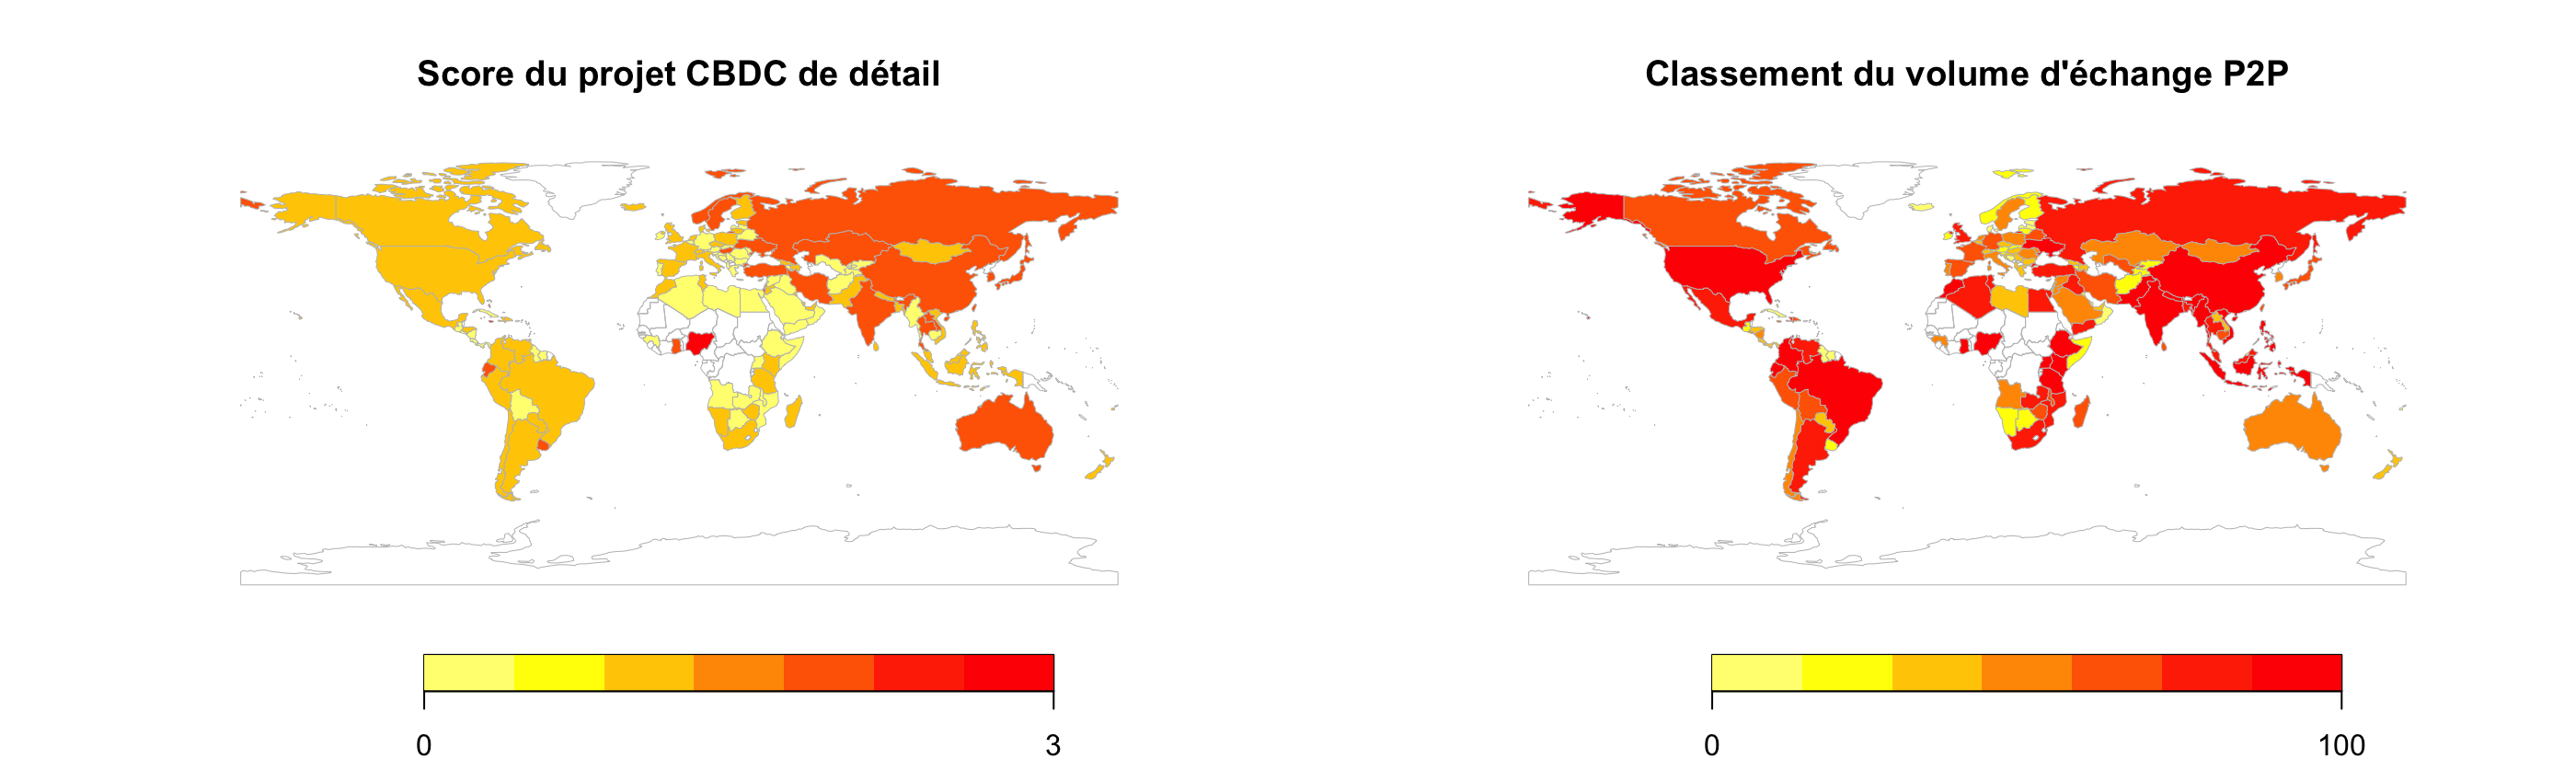
\includegraphics[width=1.5\linewidth]{Carte du monde.png}
    \caption{Comparaison entre l'adoption des cryptomonnaies d'échanges pair-à-pair et celle des MNBC de détail de 140 pays}
    \label{fig:COMPA}
\end{figure}

\begin{figure}[htbp]
    \centering
    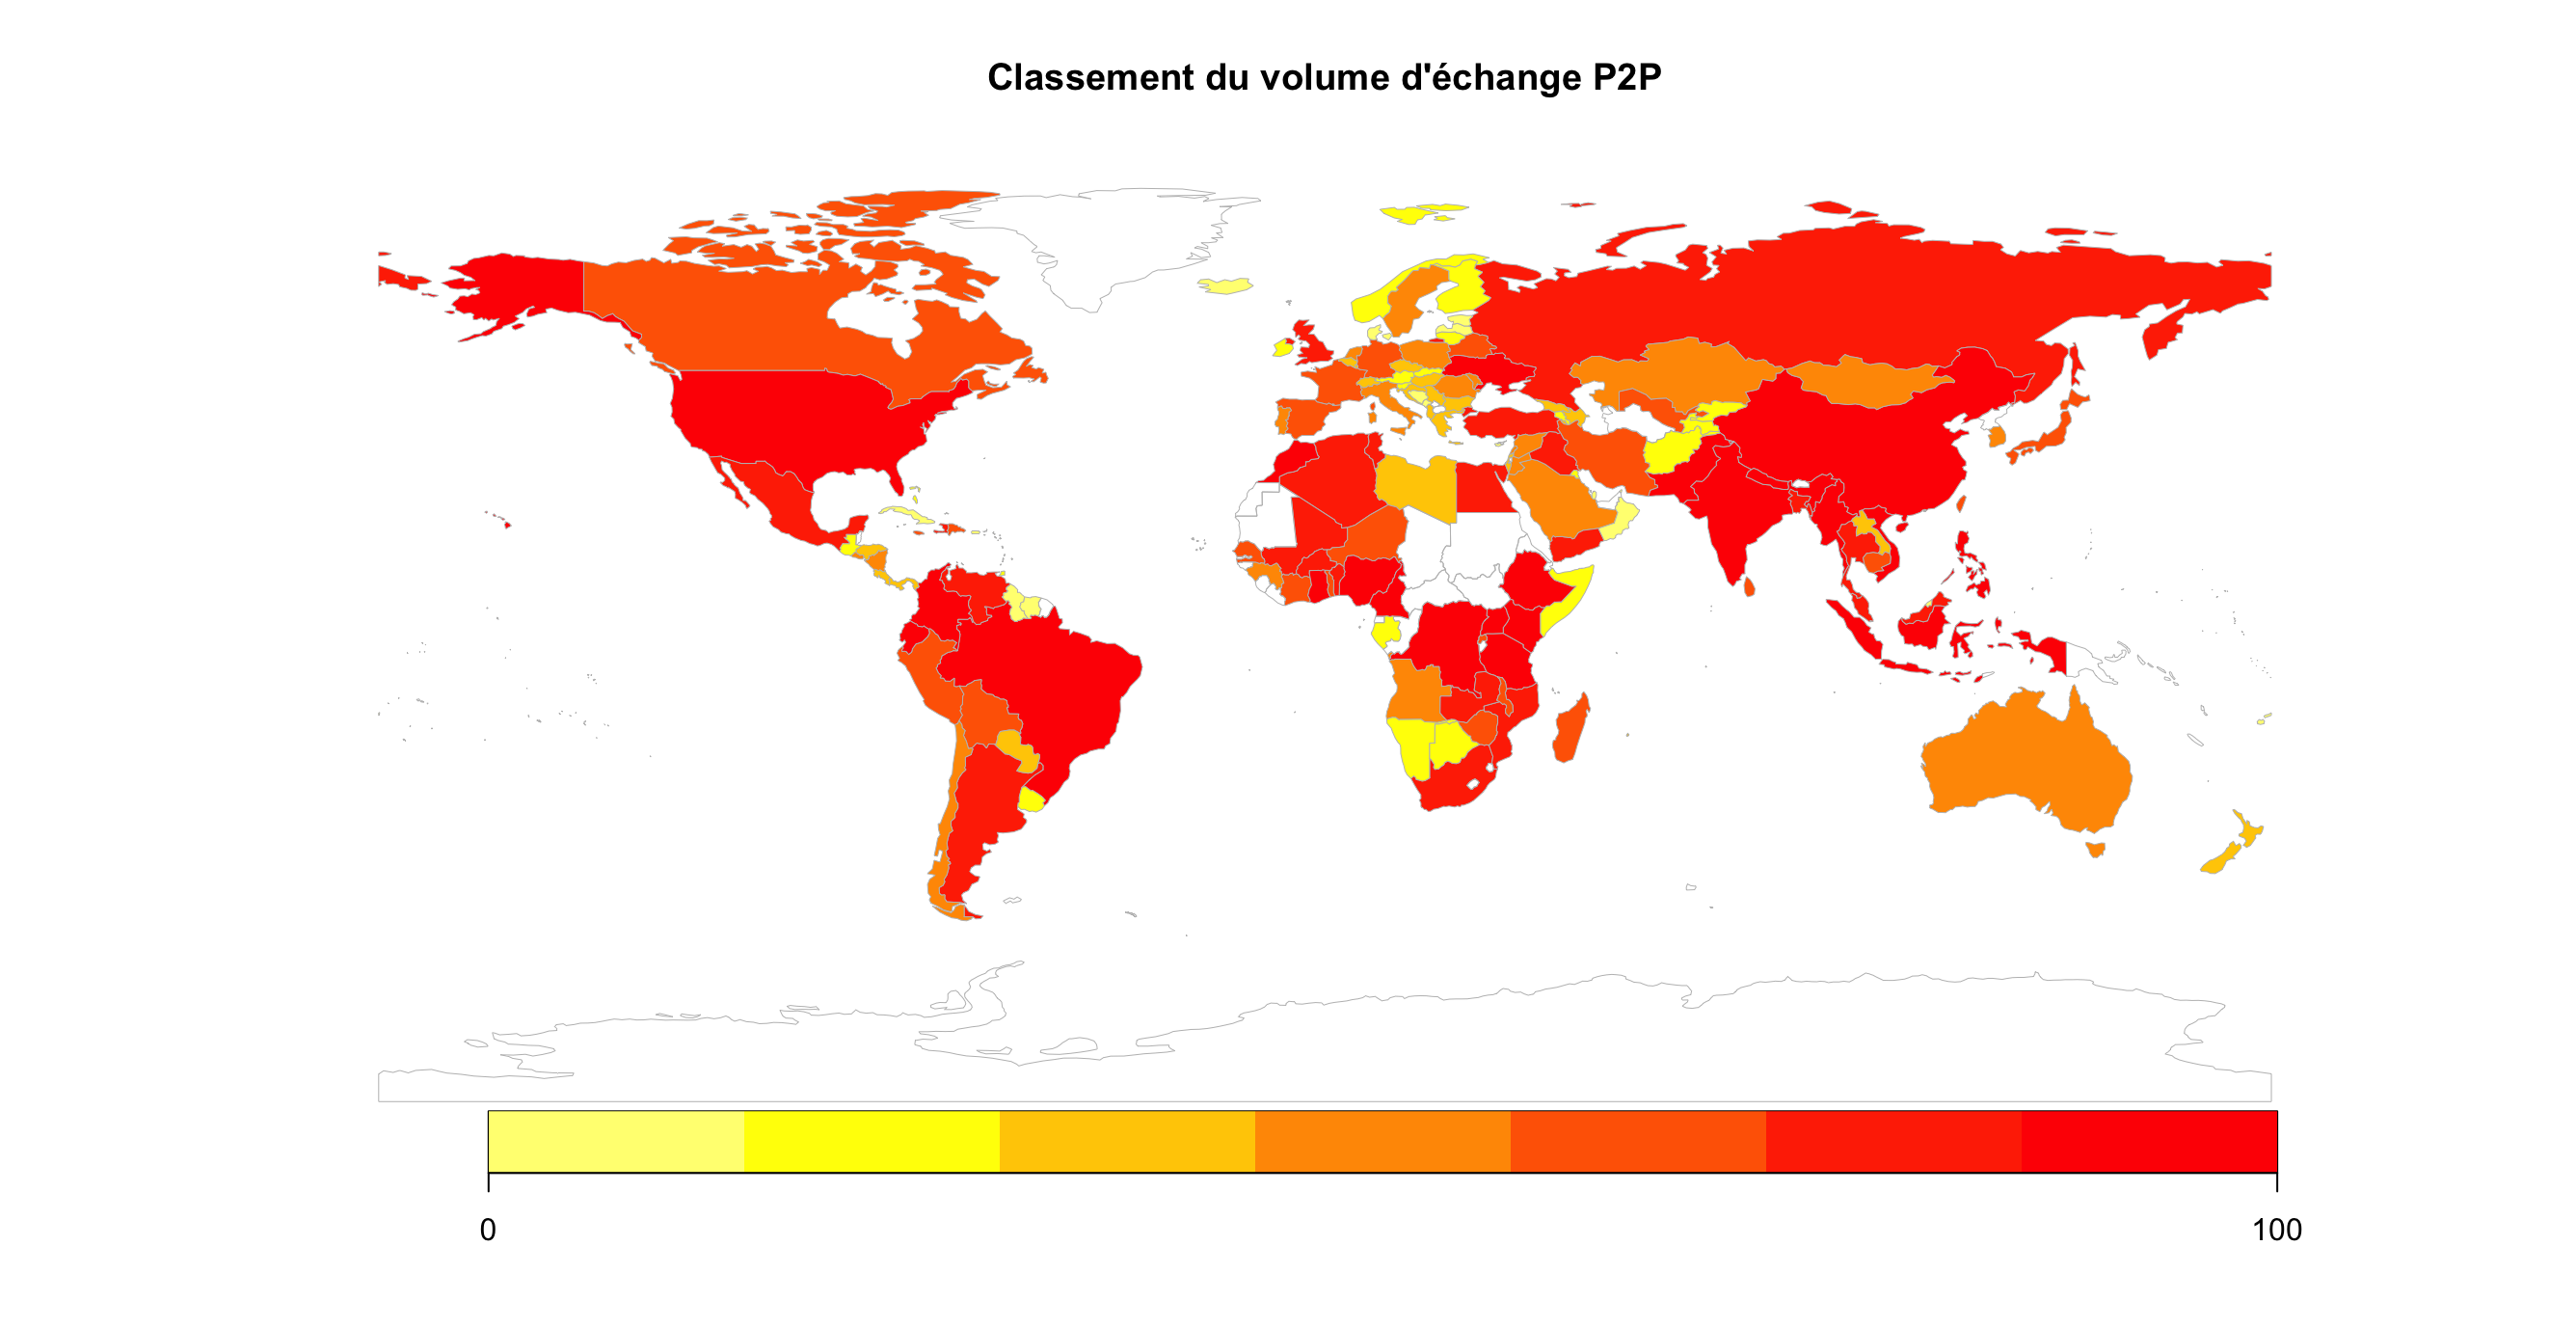
\includegraphics[width=1\linewidth]{P2P.png}
    \caption{Niveau adoption des cryptomonnaies pair-à-pair par pays en 2023 (\href{https://www.chainalysis.com/}{Chainalysis})}
    \label{fig:P2P}
\end{figure}


\clearpage
\begin{figure}
    \centering
    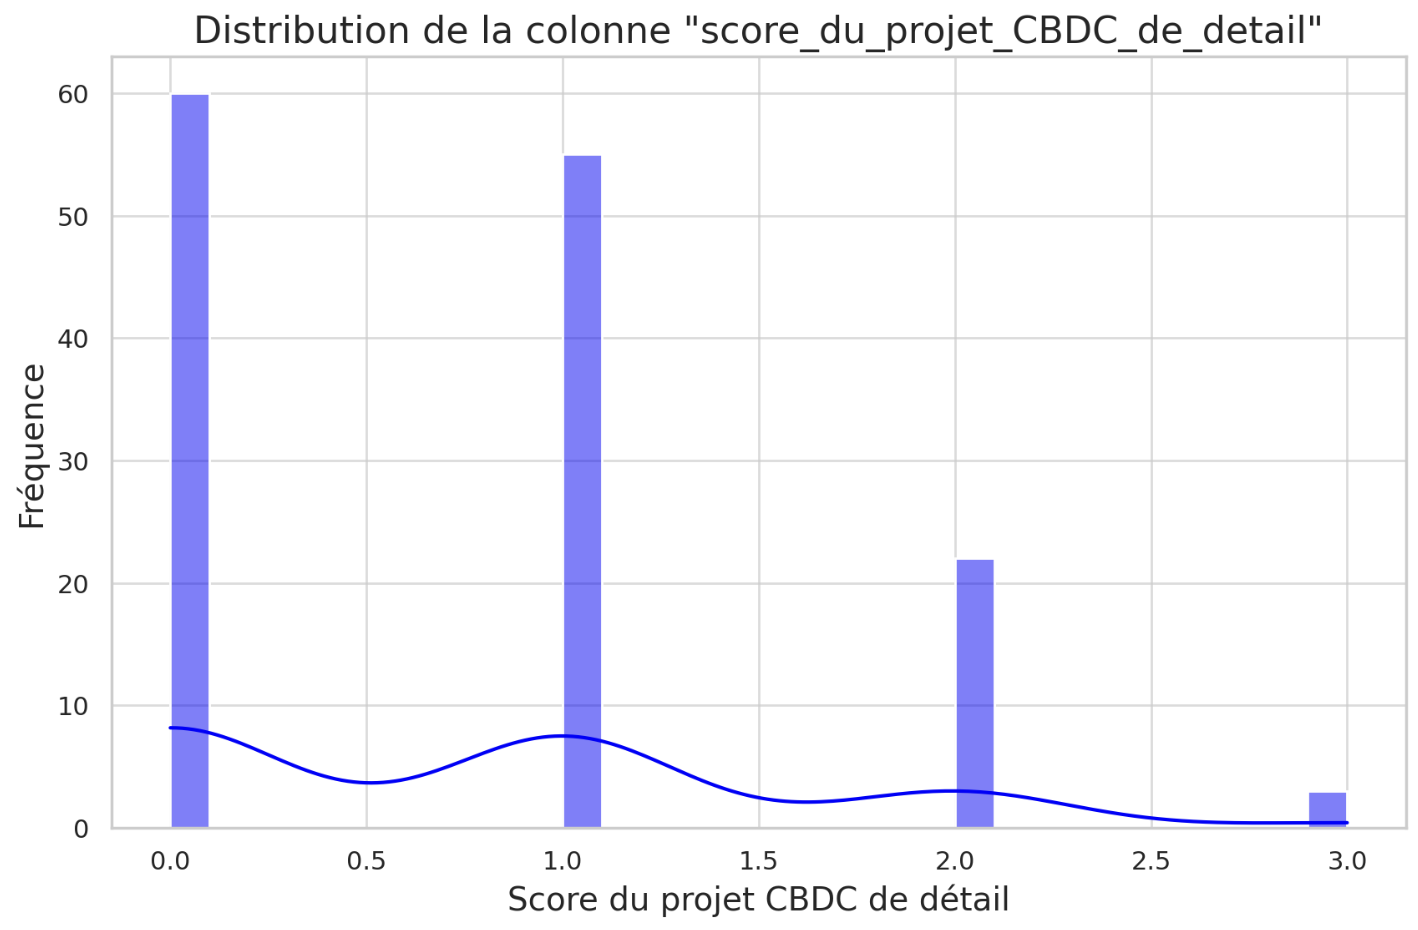
\includegraphics[width=0.7\linewidth]{Graphique CBDC.png}
    \caption{Diagrame de répartition par score par score d'avancement de MNBC de détail}
    \label{fig:graphique-MNBC}
\end{figure}

\begin{figure}
    \centering
    \includegraphics[width=0.5\linewidth]{Boite à moustache MNBC de détail.png}
    \caption{Distribution des scores d'avancement parmi les pays}
    \label{fig:Boite-a-mousatche-MNBC}
\end{figure}


\begin{figure}
    \centering
    \includegraphics[width=0.8\linewidth]{Fréquence CBDCD.png}
    \caption{Fréquences de MNBC de détail}
    \label{fig:Frequences de MNBC de détail}
\end{figure}

\clearpage


\begin{figure}
    \centering
    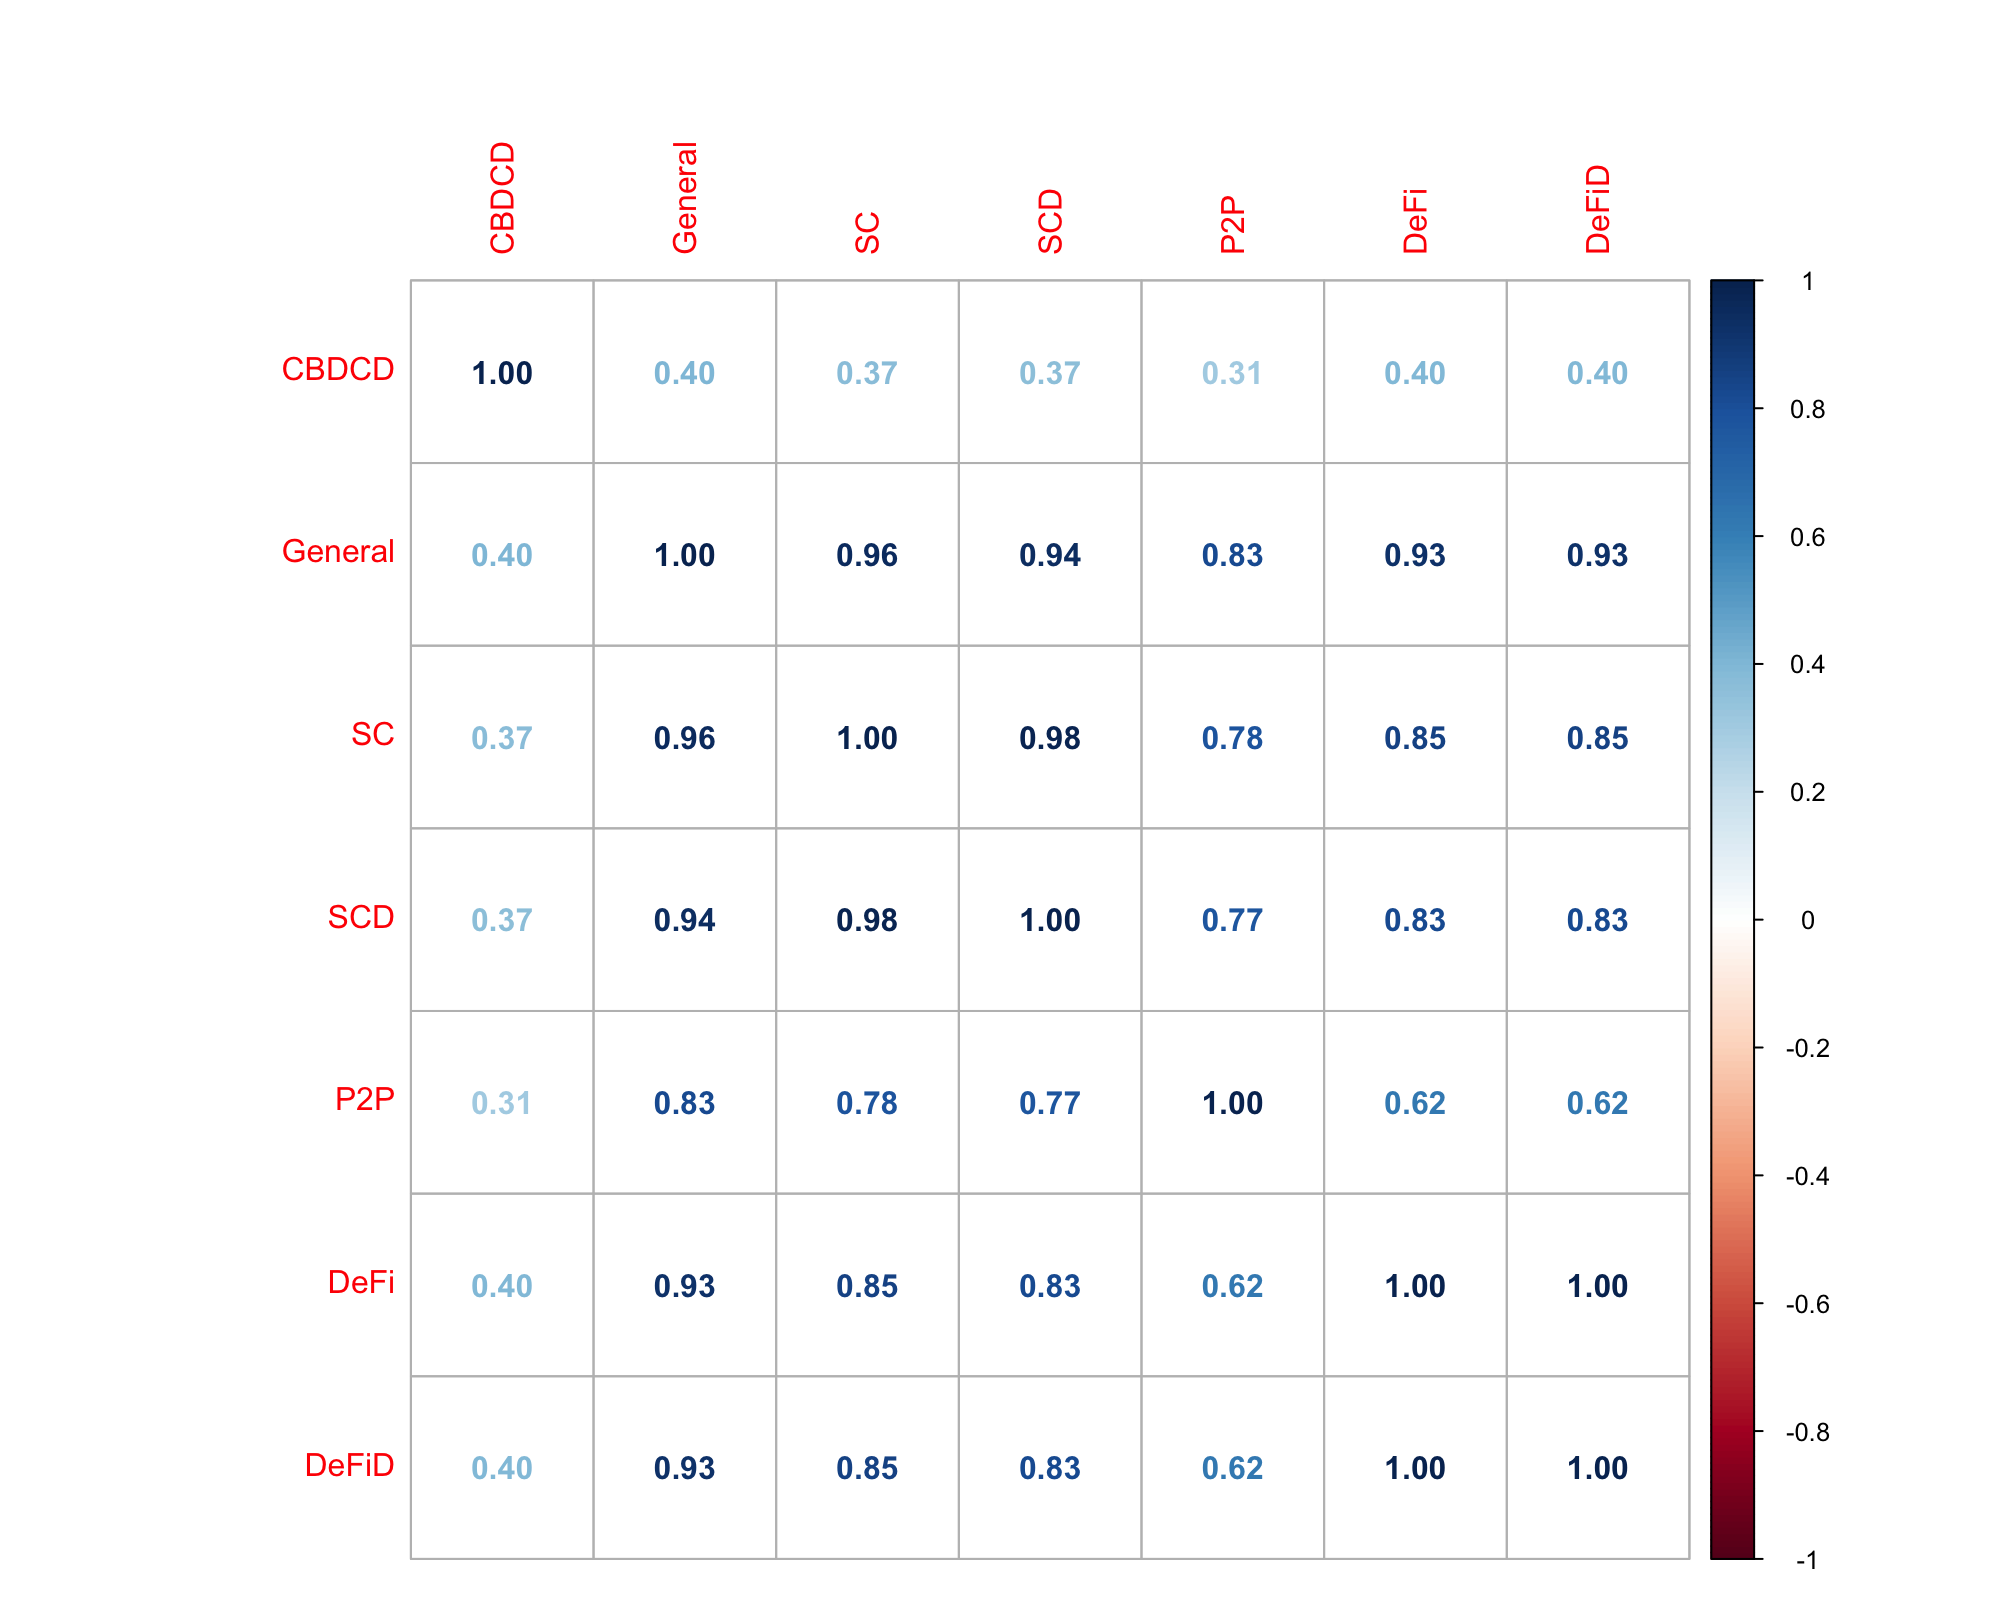
\includegraphics[width=1\linewidth]{Corr CBDC_Crypto.png}
    \caption{Matrice de corrélation 1}
    \label{fig:Correlation 1}
\end{figure}



\begin{figure}
    \hspace{-0.9cm}
    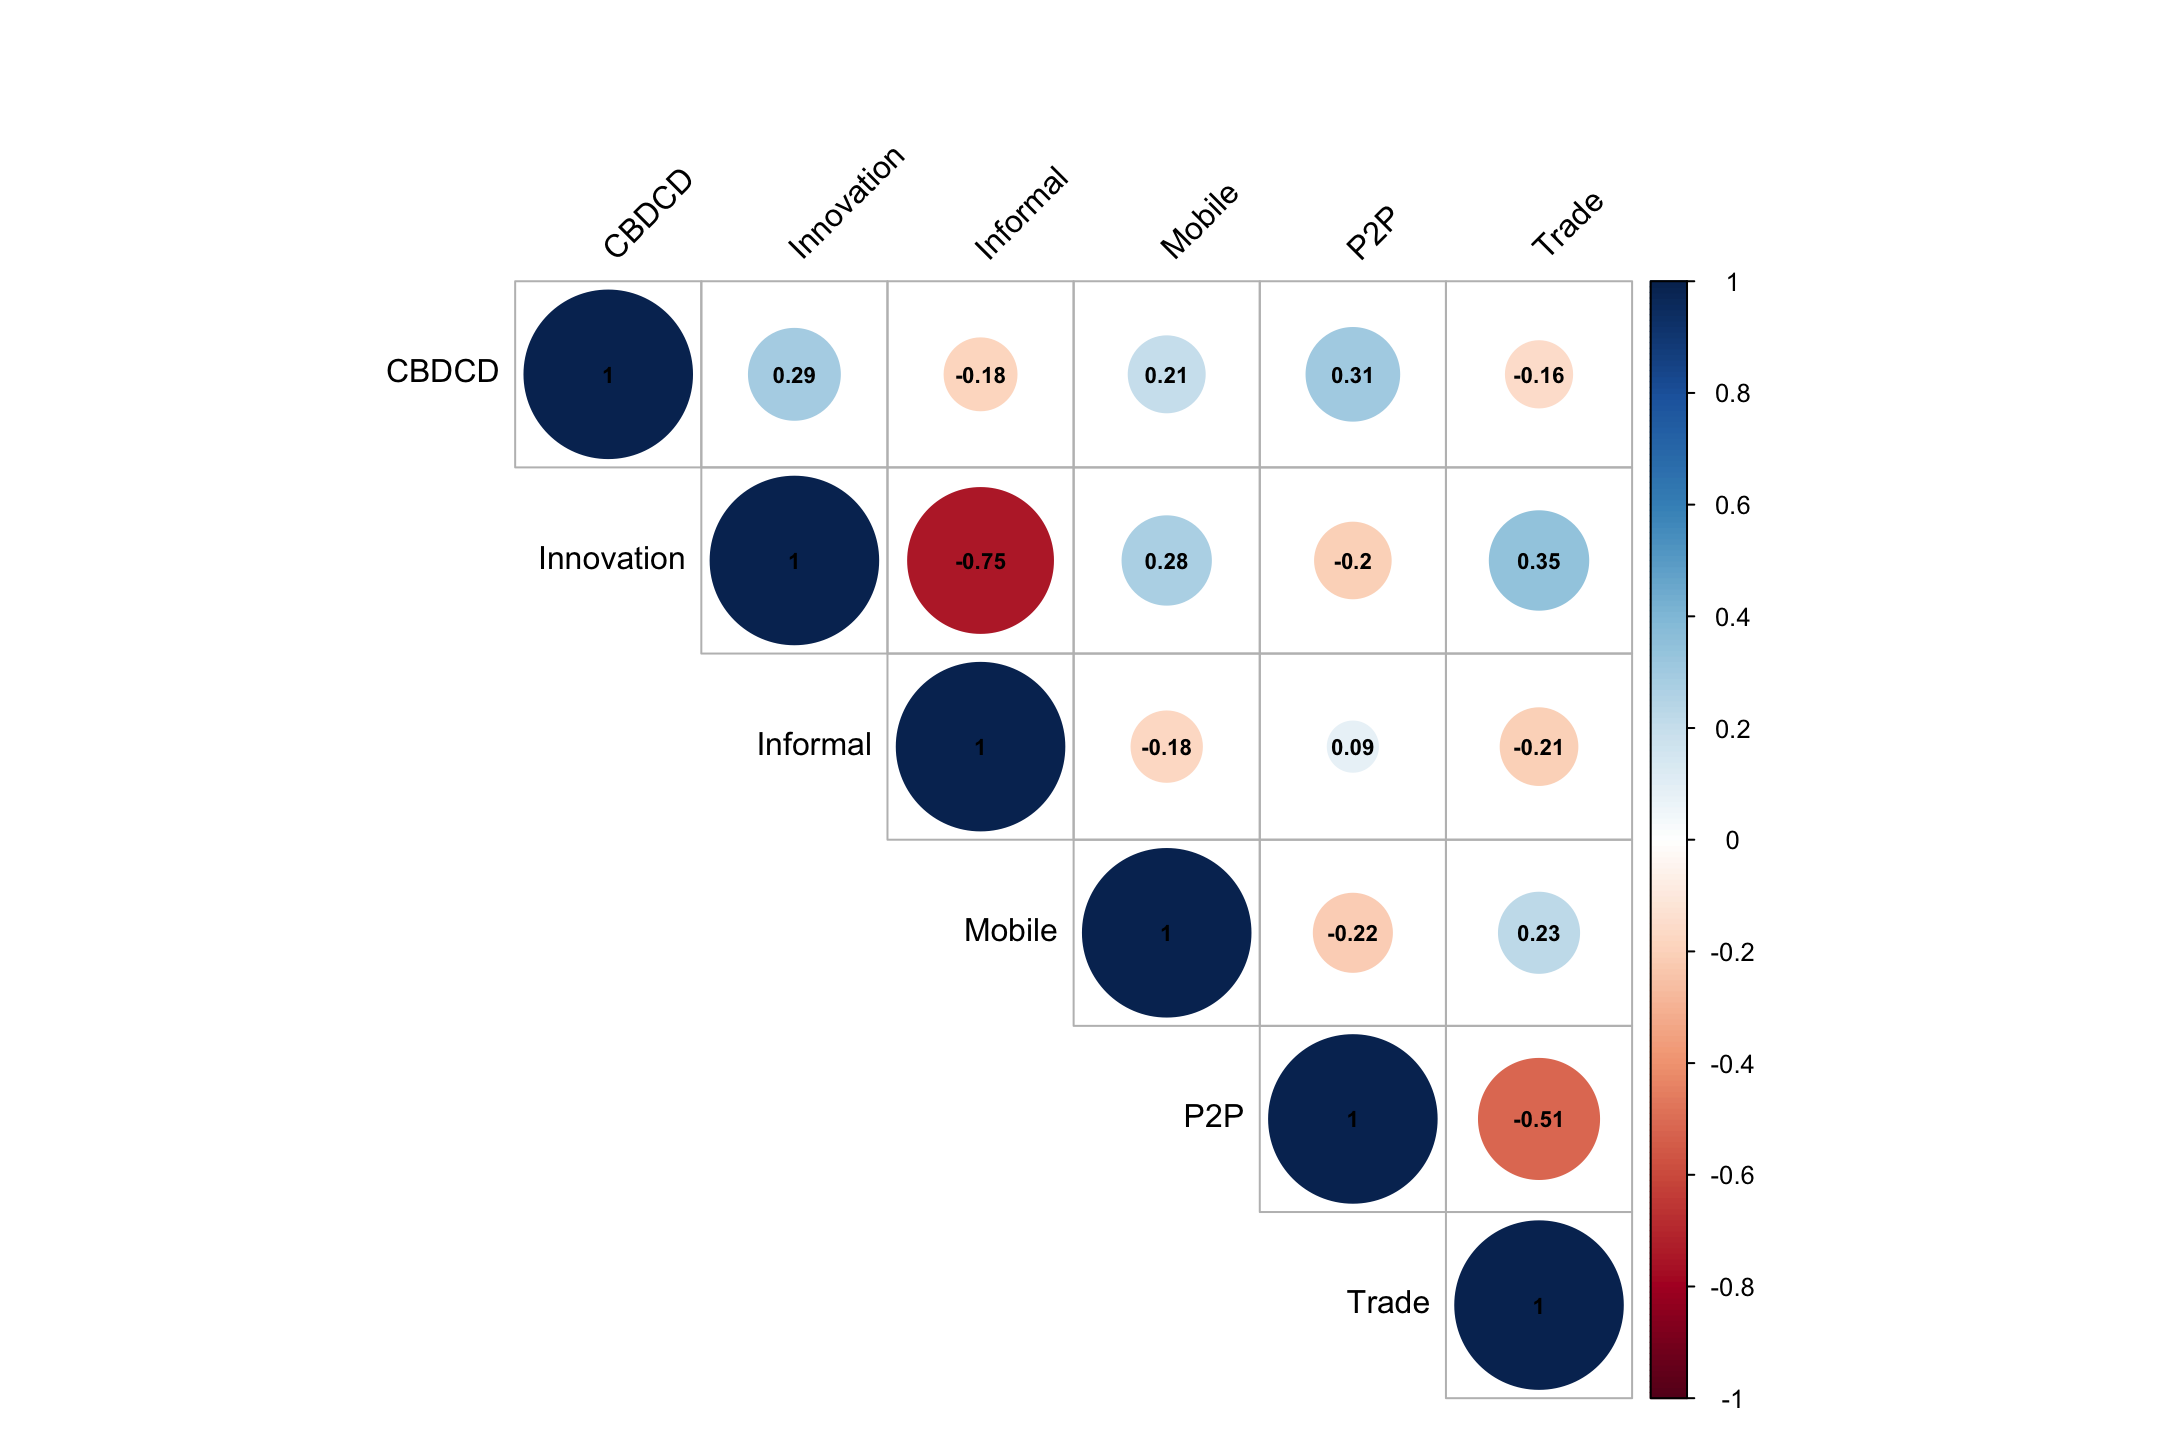
\includegraphics[width=1.2\linewidth]{Corr_Total 2.png}
    \caption{Matrice de corrélation 2}
    \label{fig:Correlaion 2}
\end{figure}

\clearpage

\begin{figure}
    \centering
    \includegraphics[width=1\linewidth]{Boite à moustache.png}
    \caption{Distribution des classements en volume d'échanges pair-à-pair par score}
    \label{fig:boxplot}
\end{figure}


\begin{figure}
    \centering
    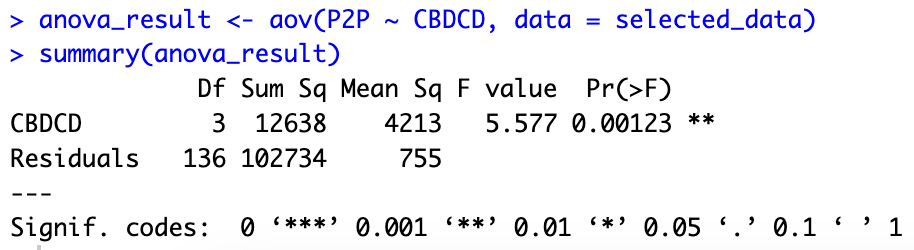
\includegraphics[width=0.8\linewidth]{Anova .png}
    \caption{Analyse de la variance}
    \label{fig:Anova}
\end{figure}

\begin{figure}
    \centering
    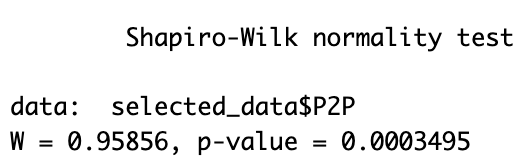
\includegraphics[width=0.8\linewidth]{Shapiro-Wilk.png}
    \caption{Test de normalité}
    \label{fig:Test de normalité de Shapiro-Wilk}
\end{figure}

\clearpage

\begin{figure}
    \centering
    \includegraphics[width=1\linewidth]{Validation croisée.png}
    \caption{Validation croisée}
    \label{fig:validation croisee}
\end{figure}


\begin{figure}
    \centering
    \includegraphics[width=1\linewidth]{TAB AUER Corrélation.png}
    \caption{Tableau de Corrélation des varibales (Auer, 2023 \cite{RePEc:bis:biswps:880})}
    \label{fig:Tableau_de_Corrélation_des_varibales}
\end{figure}

\clearpage

\begin{figure}
    \centering
    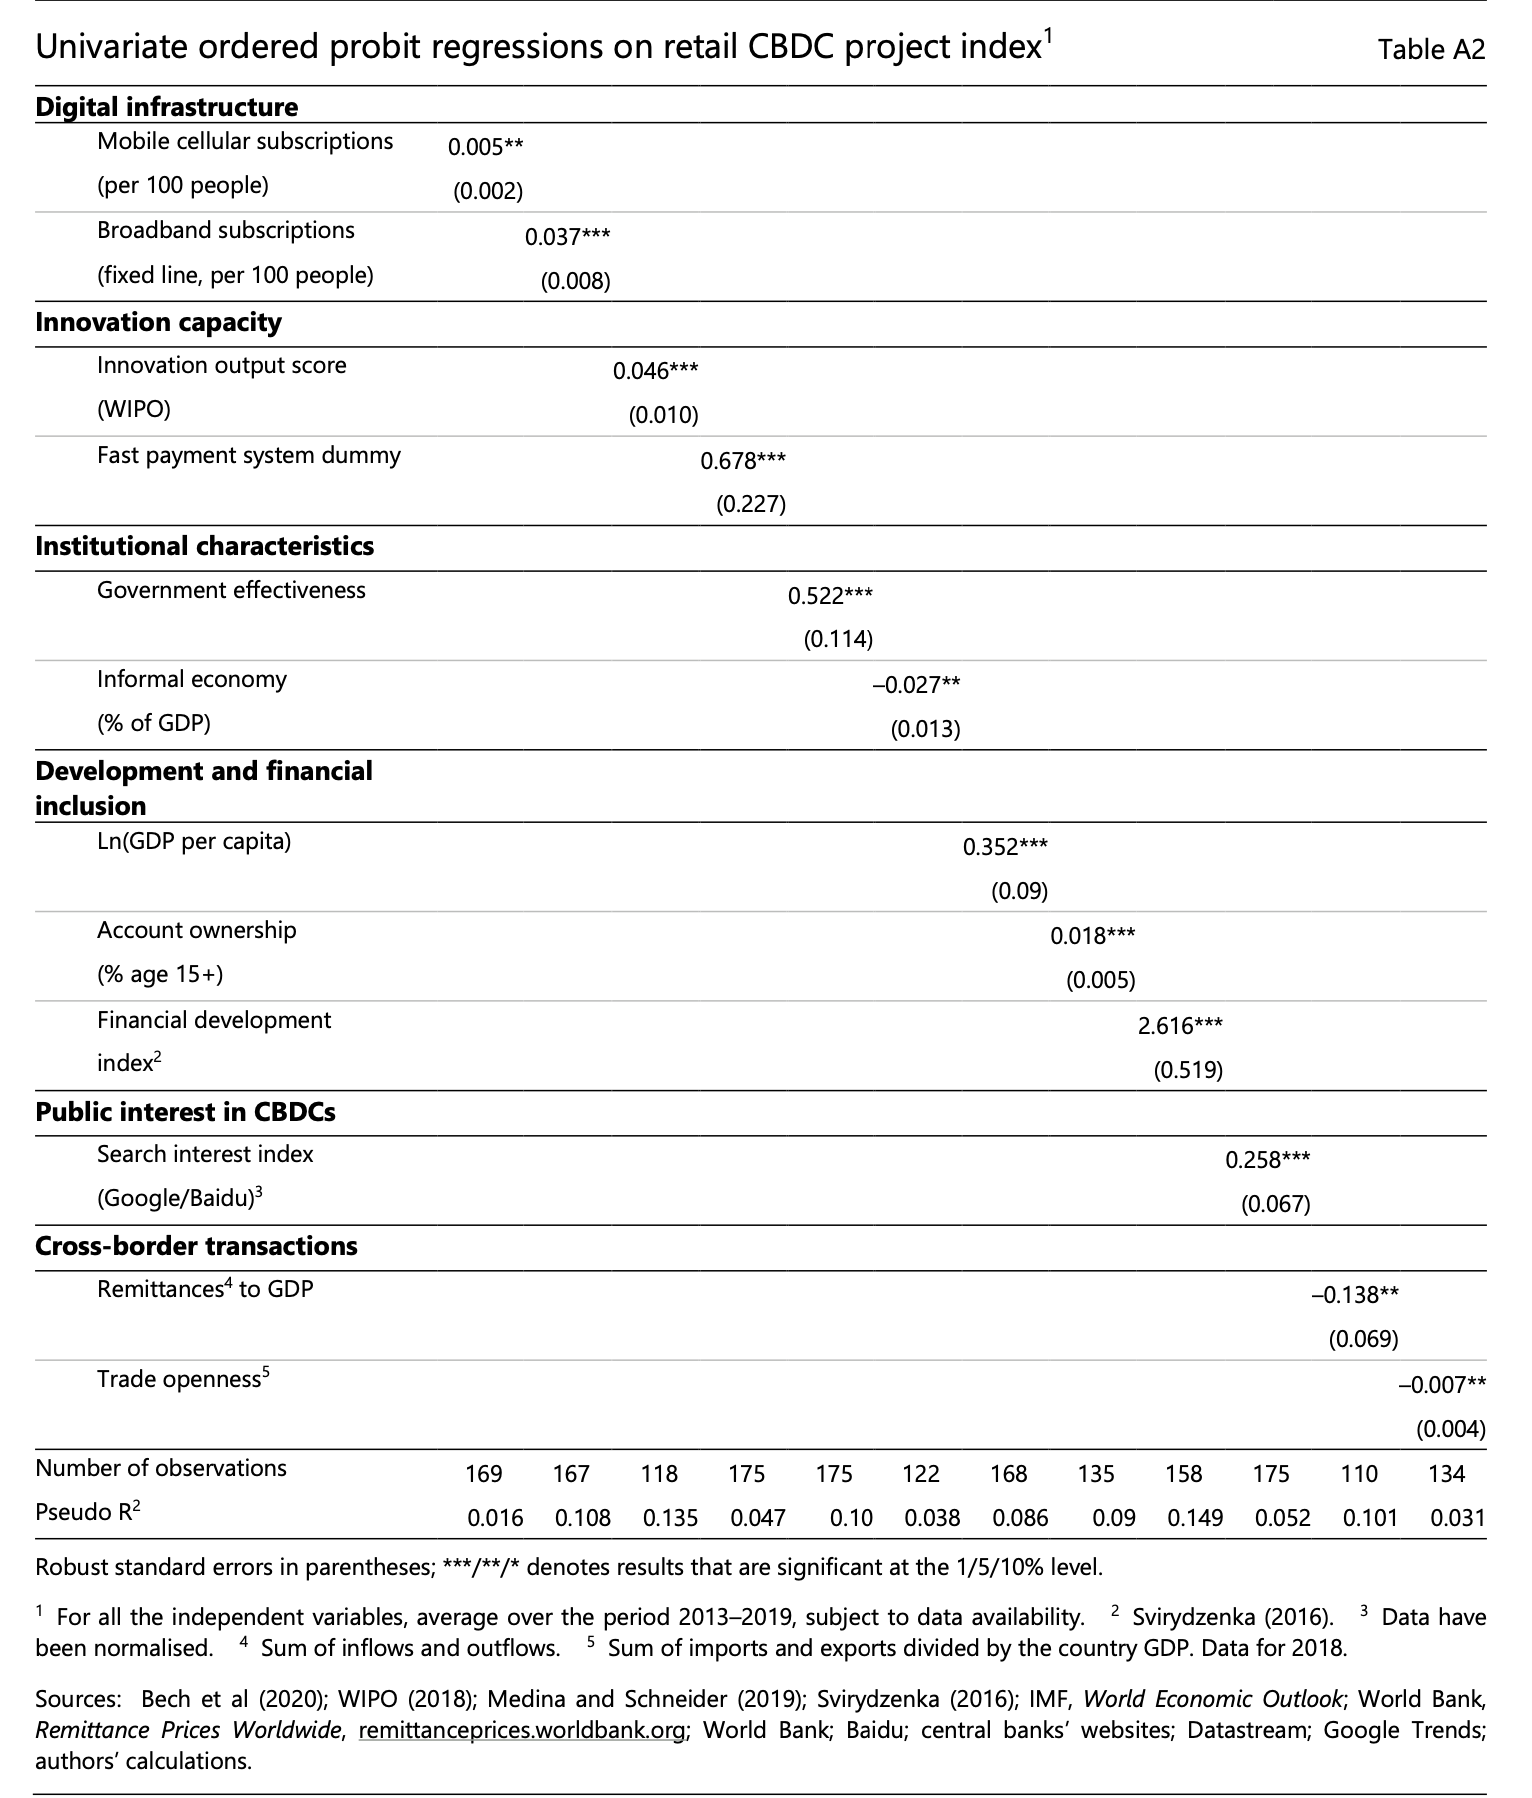
\includegraphics[width=0.8\linewidth]{TAB AUER Univariate .png}
    \caption{Regression Probit Ordonnée Univariée (Auer, 2023 \cite{RePEc:bis:biswps:880})}
    \label{fig:Regression-Probit-Ordonnée-Univariée}
\end{figure}

\begin{figure}
    \centering
    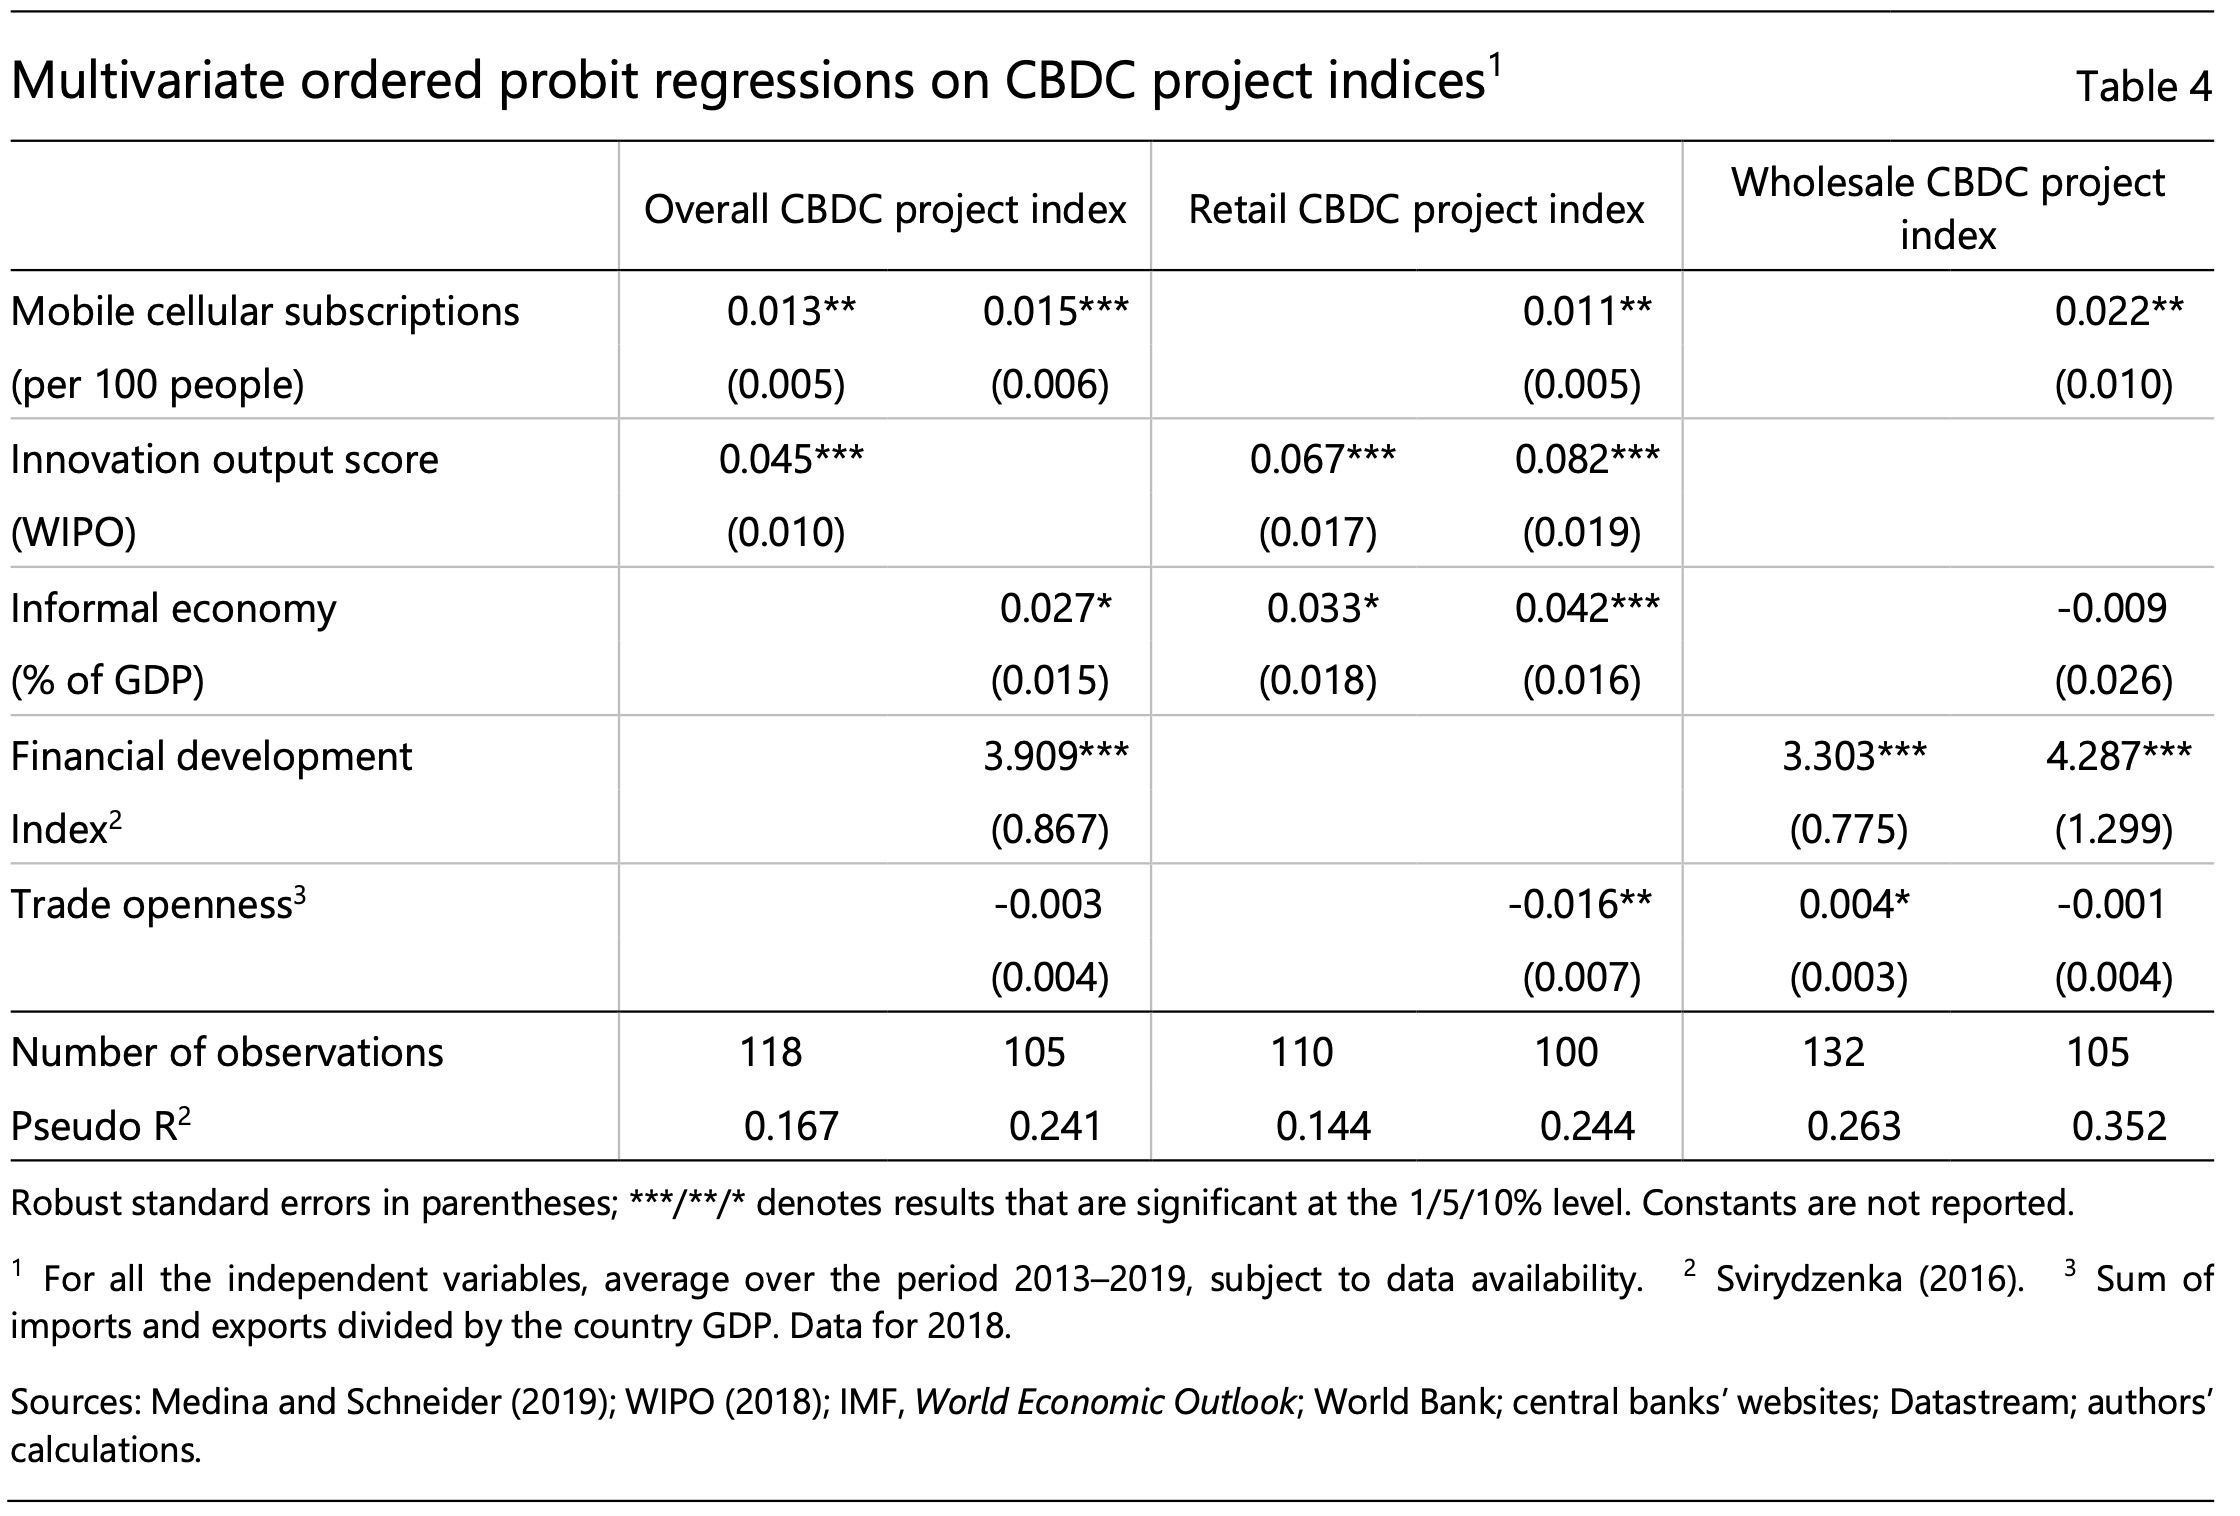
\includegraphics[width=0.8\linewidth]{TAB AUER Ordered.png}
    \caption{Regression Probit Ordonnée Multivariée (Auer, 2023 \cite{RePEc:bis:biswps:880})}
    \label{fig:Regression_Probit_Ordonnée_Multivariée}
\end{figure}

\clearpage

\begin{figure}
    \centering
    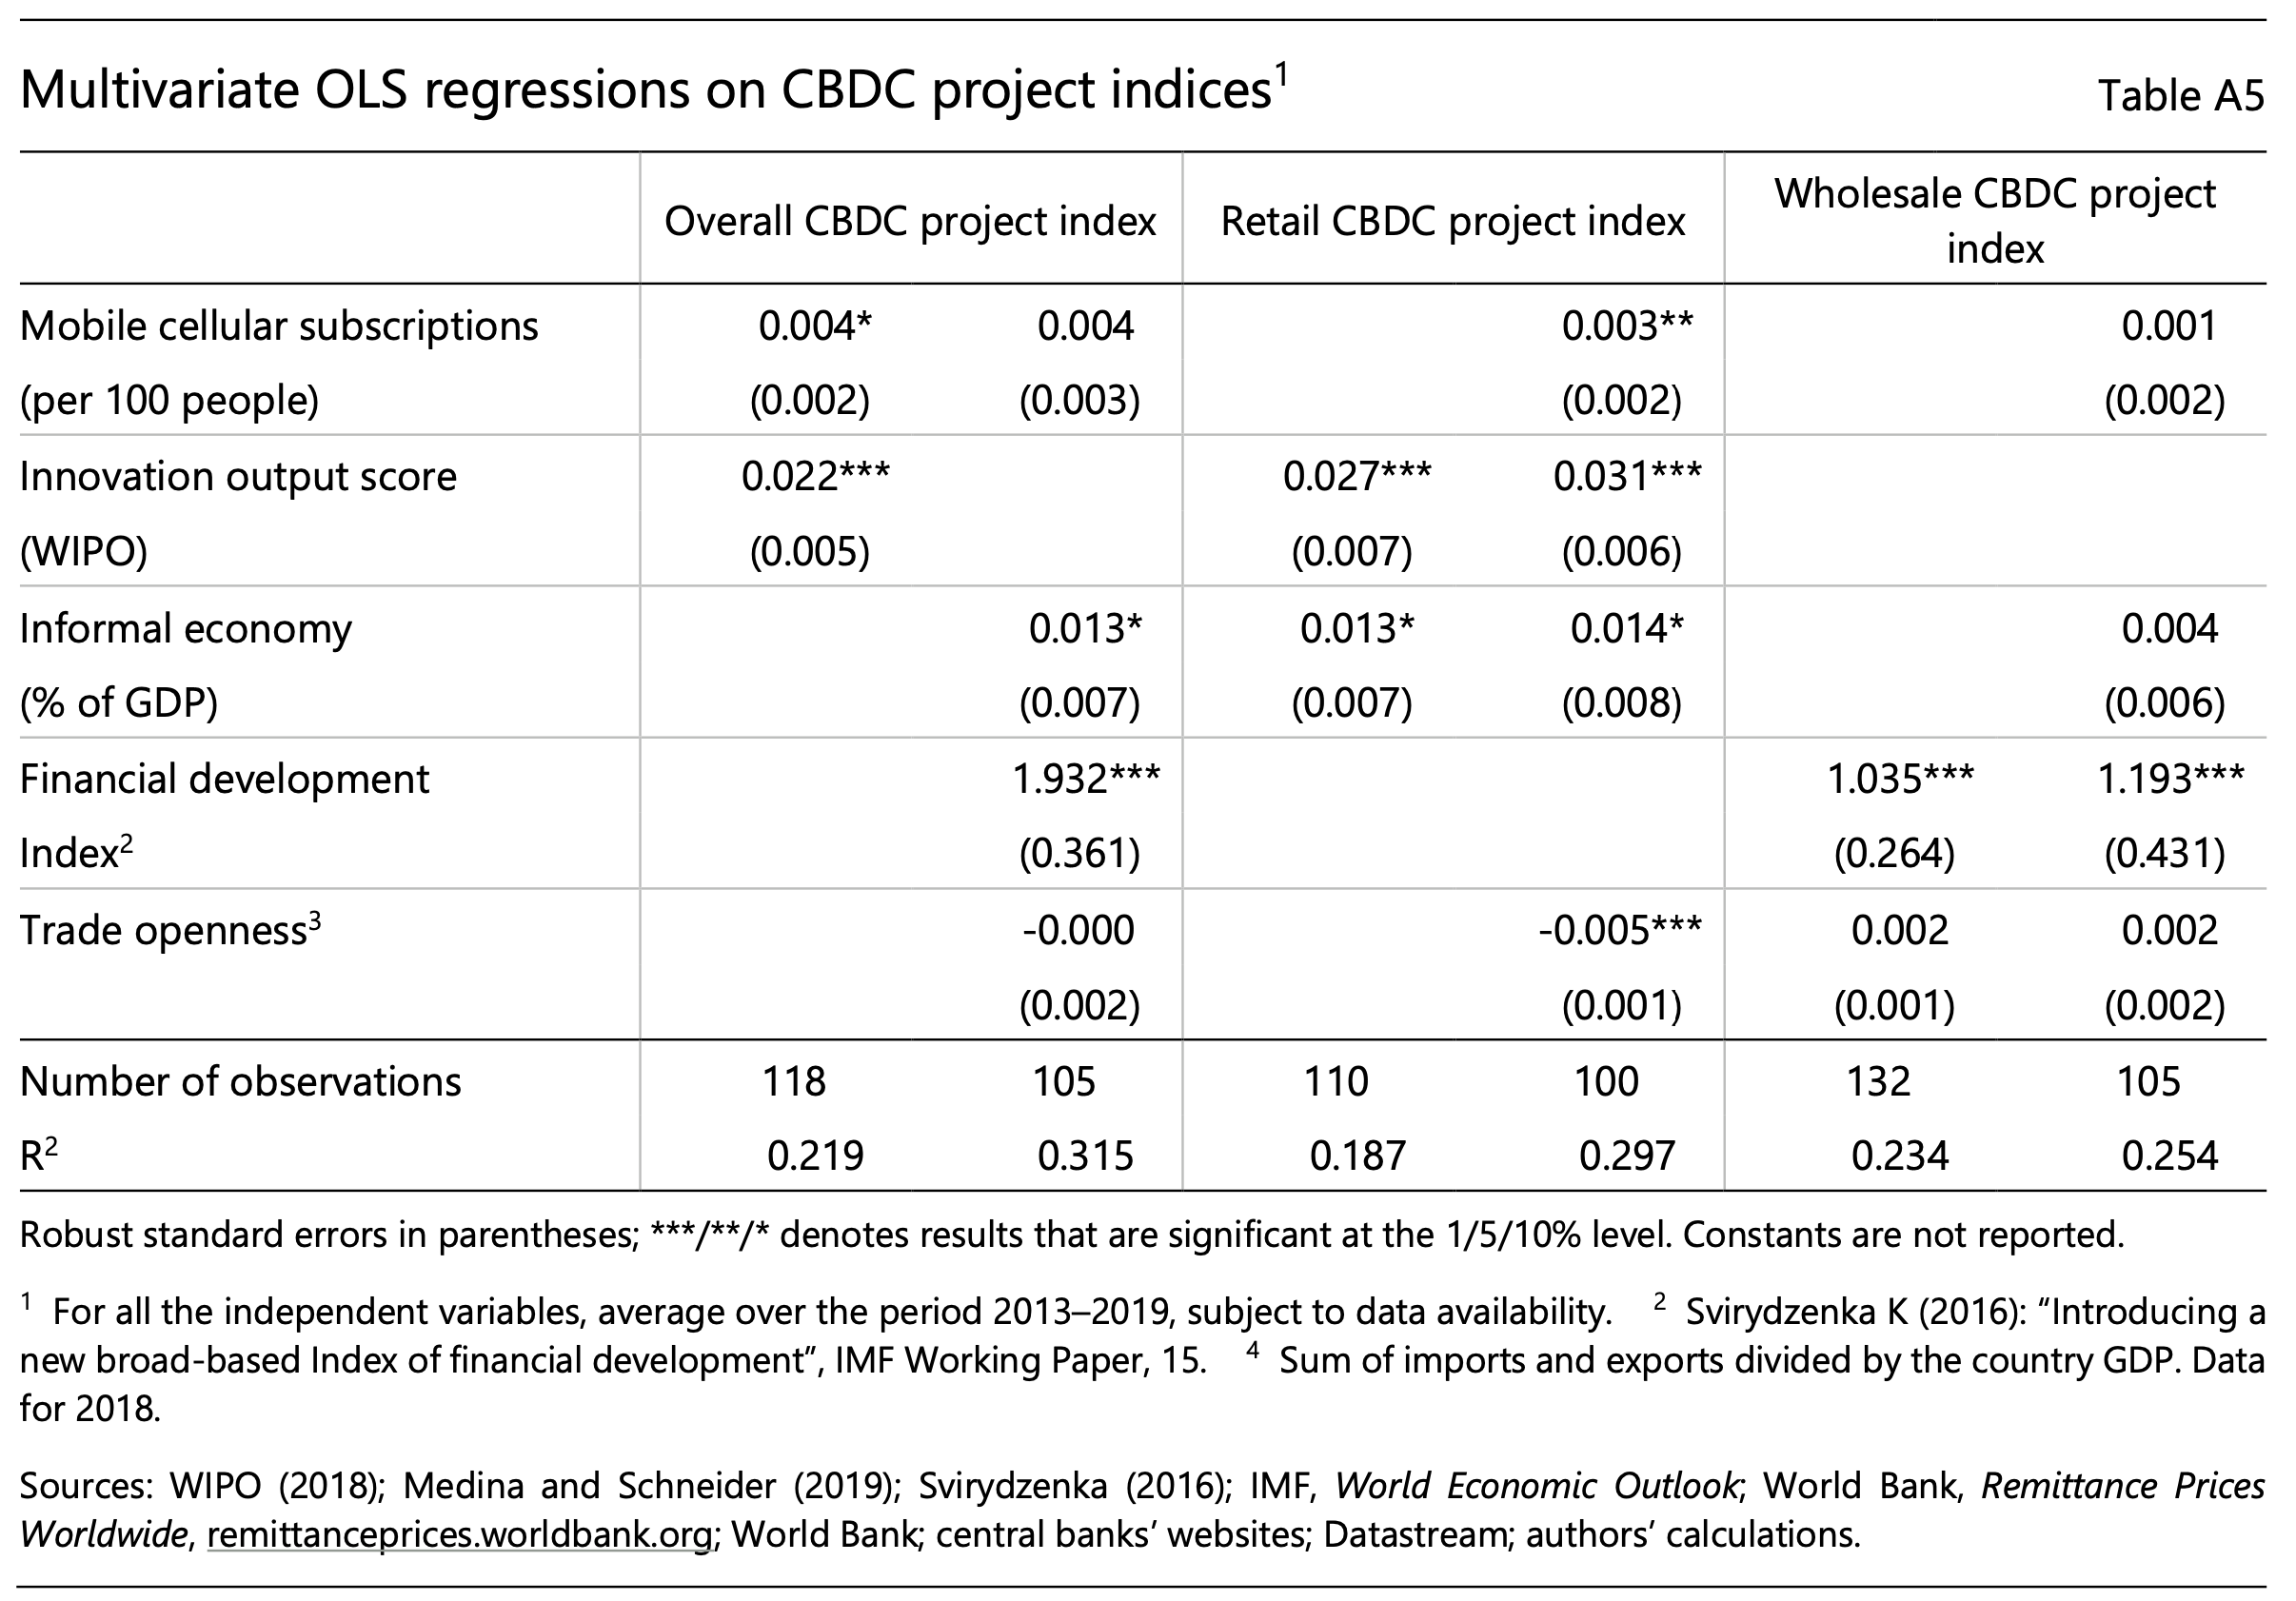
\includegraphics[width=1\linewidth]{TAB AUER OLS Multivariate.png}
    \caption{Regression OLS Multivariée (Auer, 2023 \cite{RePEc:bis:biswps:880})}
    \label{fig:Regression_OLS_Multivariée}
\end{figure}

\begin{table}[!htbp] \centering 
  \caption{Regressions en Probit ordonné} 
  \label{} 
\begin{tabular}{@{\extracolsep{5pt}}lccc} 
\\[-1.8ex]\hline 
\hline \\[-1.8ex] 
 & \multicolumn{3}{c}{\textit{Variable dépendante:}} \\ 
\cline{2-4} 
\\[-1.8ex] & \multicolumn{3}{c}{Score du projet MNBC de détail} \\ 
\\[-1.8ex] & (1) & (2) & (3)\\ 
\hline \\[-1.8ex] 
 Crypto P2P & 0.013$^{***}$ & 0.015$^{***}$ & 0.017$^{***}$ \\ 
  & (0.003) & (0.004) & (0.004) \\ 
  & & & \\ 
 Economie informelle &  & $-$0.016$^{**}$ &  \\ 
  &  & (0.008) &  \\ 
  & & & \\ 
 Innovation &  &  & 0.032$^{***}$ \\ 
  &  &  & (0.008) \\ 
  & & & \\ 
\hline \\[-1.8ex] 
Observations & 140 & 127 & 122 \\ 
Log Likelihood & $-$147.256 & $-$132.107 & $-$120.528 \\ 
\hline 
\hline \\[-1.8ex] 
\textit{Note:}  & \multicolumn{3}{r}{$^{*}$p$<$0.1; $^{**}$p$<$0.05; $^{***}$p$<$0.01} \\ 
\end{tabular} 
\end{table}

\clearpage

\printbibliography
\end{document}